\documentclass[12pt]{article}
\usepackage[T1]{fontenc}
\usepackage{calc}
\usepackage{setspace}
\usepackage{multicol}
\usepackage{fancyheadings}
\usepackage[round]{natbib}

\usepackage{graphicx}
\usepackage{color}
\usepackage{rotating}
\usepackage{verbatim}
\usepackage{array}
\usepackage{multirow}

\setlength{\voffset}{-0.25in}
\setlength{\topmargin}{0pt}
\setlength{\hoffset}{0pt}
\setlength{\oddsidemargin}{0pt}
\setlength{\headheight}{0pt}
\setlength{\headsep}{.4in}
\setlength{\marginparsep}{0pt}
\setlength{\marginparwidth}{0pt}
\setlength{\marginparpush}{0pt}
\setlength{\footskip}{.1in}
\setlength{\textwidth}{6.5in}
\setlength{\textheight}{9.25in}
\setlength{\parskip}{0pc}

\renewcommand{\baselinestretch}{1.5}

\newcommand{\bi}{\begin{itemize}}
\newcommand{\ei}{\end{itemize}}
\newcommand{\be}{\begin{enumerate}}
\newcommand{\ee}{\end{enumerate}}
\newcommand{\bd}{\begin{description}}
\newcommand{\ed}{\end{description}}
\newcommand{\prbf}[1]{\textbf{#1}}
\newcommand{\prit}[1]{\textit{#1}}
\newcommand{\beq}{\begin{equation}}
\newcommand{\eeq}{\end{equation}}
\newcommand{\bdm}{\begin{displaymath}}
\newcommand{\edm}{\end{displaymath}}
\newcommand{\script}[1]{\begin{cal}#1\end{cal}}
\newcommand{\h}[1]{\hat{#1}}
\newcommand{\ds}{\displaystyle}
\newcommand{\citee}[1]{\citet*{#1}}

\newcommand{\app}
{
\appendix
}

\newcommand{\appsection}[1]
{
\let\oldthesection\thesection
\renewcommand{\thesection}{Appendix \oldthesection}
\section{#1}\let\thesection\oldthesection
\renewcommand{\theequation}{\thesection\arabic{equation}}
\setcounter{equation}{0}
}

\pagestyle{fancyplain}
\lhead{}
\chead{A Life Insurance Deterrent to Risky Behavior in Africa}
\rhead{\thepage}
\lfoot{}
\cfoot{}
\rfoot{}

\begin{document}

\begin{titlepage}
\begin{singlespace}
\title{A Life Insurance Deterrent to Risky Behavior in Africa}
\date{\today}
\author{
Pedro de Araujo\footnote{\textit{Mailing address}: 14 E. Cache La Poudre Street, Colorado Springs, CO  80903.  \textit{Phone}: (719)389-6470.\newline  \textit{E-mail}: Pedro.deAraujo@ColoradoCollege.edu.}\\Department of Economics and Business\\Colorado College
\and
James Murray\footnote{\textit{Mailing address}: 1725 State St., La Crosse, WI  54601. \textit{Phone}: (608)406-4068.\newline  \textit{E-mail}: murray.jame@uwlax.edu.}\\Department of Economics\\University of Wisconsin - La Crosse
}

\maketitle

\thispagestyle{empty}

\abstract{The spread of HIV and AIDS and risky sexual behavior continues to be a problem in Sub-Saharan African countries despite government measures to educate people on the risk and severity of the disease and measures to promote safe sex practices such as making condoms readily available at reduced or no cost.  We examine whether people decide to engage in risky sexual behavior due to low income and low life expectancy.  Sub-Saharan Africa is characterized by conditions that significantly reduce life expectancy such as unsanitary conditions prevalent in poverty stricken areas, inaccessibility to health care, and dangerous working conditions such as those in very poor mining regions.  Moreover, since income per capita in these countries is very low, the opportunity cost associated with dying from AIDS and foregoing future consumption is very low.  We examine how a government provided life insurance benefit may be an effective means of deterring risky sexual behavior.  To evaluate this policy prescription we develop a life-cycle model with personal and family consumption and endogenous probability of survival.  In the model, agents can receive life insurance benefits if their death is not the result of AIDS.  We demonstrate that excessive risky behavior does result from low life expectancy and low levels of income and illustrate the conditions for which the life insurance benefit can replicate the effects of higher income and life expectancy, deterring risky sexual behavior and reducing the spread of HIV/AIDS.} \newline

\noindent \textit{Keywords}: AIDS, life-cycle, life expectancy. \\
\noindent \textit{JEL classification}: H51, I18, I38.
\end{singlespace}
\end{titlepage}

\newpage

\section{Introduction}\label{s:intro}

AIDS is an incurable disease that kills individuals during their most productive years and is most often transmitted through consensual, unprotected sexual encounters.  According to the most recent HIV epidemic update (\citee{UNA2009}), the worldwide number of HIV infections in 2008 was between 31 to 36 million and 2 million people worldwide died as a result of AIDS.  Sub-Saharan Africa, the epicenter of the pandemic, is responsible for approximately two thirds of all infections and over 70\% of all deaths, and the great majority of infections in sub-Saharan Africa is due to heterosexual sex.  HIV prevalence among adults in sub-Saharan Africa is approximately 5.2\%, whereas the worldwide prevalence among adults is only 0.8\%.  In some sub-Saharan countries the pandemic is particularly bad: the adult HIV prevalence reaches 26.1\% in Swaziland, 23.2\% in Lesotho, and 15.2\% in Zambia.  These numbers are not projected to decrease any time soon.

There has been a substantial body of research, empirical and theoretical, on the effects of HIV on economic growth and development.  \citee{RVP2002} demonstrate that policies to reduce HIV incidence in the short-run are particularly important as the epidemic reduces private savings and capital accumulation.  In an early study, \citee{O1992} uses a two sector model for 30 sub-Saharan African countries and finds a negative effect on annual real GDP growth of 1\%.  Other studies have found similar effects on economic growth of African economies, for example \citee{KDO1992}, \citee{CH1994}, \citee{Al2000}\footnote{They find a 2.6\% negative growth effect.}, \citee{B2000}, \citee{WBL2000}, \citee{WBS2001a}, \citee{WBN2001b}, and \citee{DMR2001}. When we compound a 1\% loss in real GDP growth over many years, this effect becomes very large\footnote{Many other papers have found very large long-run level effects of HIV on output, including \citee{C1993b}, \citee{CH1995}, \citee{BIDPA2000}, \citee{Arndt2003}, \citee{BDG2003}, \citee{RS2007}, \citee{RS2008}, and \citee{PDA2008}.}. In the absence of a cure or an effective prevention campaign, the evidence suggests that AIDS in sub-Saharan Africa can be a great impediment to long-run economic growth.  

The evidence above has been contested by some studies. \citee{BM1997} use data for 51 countries and find no effect of HIV on economic growth. \citee{AY2005a} constructs and simulates a model in which HIV generates two opposing effects: reduced fertility and reduced human capital. He argues that the former effect outweighs the latter implying increases in the standards of living over time. Since then, however, \citee{CGM2005} show the human capital loss effect is much greater when accounting for inter-generational transfers in schooling decisions.  This large loss in human capital is also demonstrated by \citee{HB2002} and most recently in \citee{JF2008}.  In short, there is strong evidence that HIV/AIDS is not only a health problem, but a serious economic problem in sub-Saharan Africa.

Because the main mode of HIV transmission in sub-Saharan Africa is through heterosexual sex, most public policy efforts to contain the spread of the disease focus on influencing individuals to limit engagement in unprotected sex and to be faithful to their partners.  Usually these campaigns involve educating the population on HIV/AIDS and discussing how sexual behavior increases risk of transmission.  In this paper we suggest an alternative policy approach, still aimed at influencing people's risky sexual behavior.  We investigate the efficacy of government-provided life insurance benefit payable to families for deaths that are not the result of AIDS.  We use a life-cycle optimization model to show that individuals' decisions to engage in risky sexual behavior depend negatively on income and non-HIV life expectancy.  When compared to the developed world, individuals in sub-Saharan African countries have very short life expectancies, even absent of the HIV/AIDS epidemic, and very low average levels of income per capita.  Simply put, when individuals have less to lose, they are more likely to engage in risky behavior.  We then show that a government-provided life insurance benefit payable in only for non-HIV related deaths can replicate the behavioral effects on sexual activity of having a higher income and longer life expectancy.

\section{HIV/AIDS Prevention Policy}
Between the years 1996 and 2007, the Global Fund for AIDS, Tuberculosis and Malaria (GFFATM), the World Bank's Global AIDS Programme, and the US President's Emergency Plan for AIDS Relief (PEPFAR) have disbursed \$10 billion dollars to prevention and treatment programs mostly in sub-Saharan Africa. This constitutes a forty-fold increase in funding within a decade.  Given this most recent sharp increase in funding from international organizations and developed countries (especially the United States) to support programs to combat the spread of HIV and AIDS in sub-Saharan Africa, it is important to investigate the effectiveness of such programs, and in particular, whether such programs effectively limit people's choices to engage in risky sexual activity.

A number of education campaigns target high risk groups (truck drivers, commercial sex workers, mine workers) and the general population.  The goal of these programs is to decrease risky sexual behavior through increased knowledge about the disease.  Even though there have been studies that document the success of prevention campaigns (\citee{NM1999}, \citee{EG2006}, and \citee{PD2009}), there is not much evidence, at the macro level, of substantial change in risky behavior in sub-Saharan Africa. For example, \citee{AAP2010} find that increases in HIV knowledge are associated with more condom use, but also with more pre-marital and extra-marital sex.  \citee{HE2007} argues that changing sexual behavior in sub-Saharan Africa is very difficult as it requires changing social norms.  In some countries in Africa, it is socially acceptable for males to have contingent relationships.  This creates a sexual network that can lead to a greater spread of HIV than in the situation of serial monogamy.  Other studies that have documented no real change in sexual behavior in sub Saharan Africa since the advent of the AIDS epidemic include \citee{Lin1991}, \citee{L1996}, \citee{Ng1996}, \citee{Cald1999}, \citee{Bloom2000}, \citee{Wil2003}, and \citee{Stone2004}.

In Zambia, PEPFAR reports that 23.8\% of all HIV/AIDS funding in 2007 went to prevention programmes that promote abstinence, faithfulness, and condom use through behavioral change\footnote{www.pepfar.org}. More generally, the Global Fund disbursed 31\% of its HIV budget for programs that target HIV education and prevention (\citee{GF2011}). The idea that such programs are effective in promoting safer sexual practices and, therefore, reducing the risk of HIV has been widely debated (see, for example, \citee{VD2000}, \citee{Bloom2000}, \citee{EHAP2006}, and \citee{DW2009}).  \citee{eo2007} has shown that the measured success of such campaigns in one country is possibly misidentified.  Oster finds that the fall in HIV prevalence in Uganda during the 1990s was closely tied to the price of exports; that is, the major cause of the decrease in HIV prevalence was a reduction in economic activity due to decreases in exports.  \citee{GV2001} suggests that the limited efficacy of HIV prevention campaigns may be due to that existing government expenditures on health and education in Africa are not efficient, as compared to other regions of the world.  This is likely due to mismanagement of HIV funds by local governments.

Containing HIV in sub-Saharan Africa would be much less challenging if it were possible to dissuade risky sexual behavior. Even with millions of dollars spent on campaigns that focus on improving HIV knowledge and education and increasing condom distribution, there is little evidence that behavior has substantially changed at the macro level and there is relatively little evidence that country-wide HIV prevalence has decreased as a result.  Some studies suggest the only feasible way to contain the pandemic is by creating opportunities for these countries to surpass a certain development threshold where life expectancy and wealth are increased to levels in which the incentive to engage in risky sexual practices is reduced.  \citee{eo2009} concludes furthering education campaigns would be ineffective as HIV knowledge in Africa is already very high; however, she does not propose a concrete alternative.

We investigate such an alternative policy: a government provided life insurance benefit that is payable for deaths that are not the result of AIDS.  We develop a life-cycle model where the decision to engage in risky sexual behavior is endogenous and depends on, among other things, income and life expectancy.  The model incorporates an incentive structure in the spirit of \citee{HO2010} that rewards households if males reduce their risky sexual behavior.  We focus specifically on married males that have family dependents.  Males they have been found to be the drivers of the pandemic in sub-Saharan Africa (\citee{Ulin1992}, \citee{HE2007}), which implies that everyone in sub-Saharan Africa would be at less risk of contracting HIV if males reduce their risky sexual behavior.  We calibrate the model to match data for Zambia and four other sub-Saharan African countries.

We find that this contingent life insurance can act to deter risky sexual practices in males much the same way an increase in wealth does, and depending on parameter calibrations may even replicate the relatively large deterrence effect that comes from an increase in life expectancy.  This paper is able to match some of the same qualitative predictions made by \citee{eoQJE}, but with a feasible policy prescription.

\section{Model}\label{s:model}

The focus of this paper is on married adult males who are the primary wage earner of their family and have dependent family members.  Such an agent can live up to four fifteen-year periods.  The agent is alive through the first period and faces a possibility of dying before periods 2, 3, or 4, possibly from AIDS if HIV was sexually transmitted during the previous period, or possibly from accident or another illness that is beyond the agent's control.  The first period is thought to approximate ages 20 though 34, the second period ages 35 through 49, the third period ages 50-64, and the final period ages 65 through 79.  It is therefore possible to live up to age 80 years, but since an agent can die from exogenous factors, the non-AIDS life expectancy can be far below 80.  The probability of survival to the next period depends on factors beyond the a person's control (such as accidents that can result from working in dangerous conditions or contracting non-preventable illnesses) and also a factor the agent can control, risky sexual activity.   We assume during the first three periods the agent is employed and earns wage income and in the final period he is retired.  He decides how to allocate his income between his own consumption and the consumption of his other family members.

\subsection{Preferences}

The agent's utility at time, $t$, depends on his personal consumption, $c_t$; his family's consumption, $f_t$; and the number of risky sexual partners, $m_t$.  We assume the utility function for a given period is additively separable over the consumption goods and sexual activity, so that the utility in period $t$ can be given by,
\beq \label{eq:util} u(c_t, f_t, m_t) = v(c_t, f_t) + \gamma_t w(m_t), \eeq
where $\gamma_t$ is a scale parameter that determines the relative importance of consumption and risky sexual partners.  We suppose this parameter may be different for different periods in the agent's life.  As the agent gets older we will suppose the preference for having risky sexual partners may decrease.  If $\gamma_t$ were to remain constant, the agent will optimally choose to have larger and larger numbers of risky sexual partners as he gets older since there is less lifetime consumption and income to lose if he dies from AIDS.  Since it is more common to see the opposite behavior, people typically have fewer sexual partners in a given time period as they age, it is likely that $\gamma_t$ gets smaller as $t$ gets larger.  We assume there is no close substitute for risky sexual behavior, such as monogamy or protected sexual activity, for two reasons.  First, in the context of the model there would be no implicit or explicit cost for these substitute activities.  Therefore, an agent can engage in these practices until he reaches physical limits or a satiation point.  Secondly, if safe sexual activity was a close or perfect substitute, it would be extremely unlikely or impossible that an agent would risk contracting HIV to engage in risky sexual activity.  We know that people do make this choice and take this risk, and the purpose of this paper is to examine how such decisions can be altered by changing incentives.  One way to alter the model to account for the possibility that safe sexual practices are substitutable for risky sexual activity is to simply decrease $\gamma_t$ parameters.  Setting these to zero implies safe sexual practices are perfect substitutes for risky practices, so the agent engages in no risky behavior.

The additivity assumption implies there is no substitutability between consumption of goods and sexual activity, so the agent's marginal utility for sexual activity cannot be enhanced or diminished with greater personal or family consumption.  Put another way, the agent's preferences for risky sexual activity are not related to his preferences for consumption.  Allow the utility function for personal and family consumption be given by the following constant elasticity of substitution (CES) utility function,
\beq \label{eq:utilcon} v(c_t, f_t) = \log\left( \left[\alpha \left(c_t + \epsilon\right)^{\frac{\nu-1}{\nu}} + (1-\alpha) \left(f_t + \epsilon \right)^{\frac{\nu-1}{\nu}} \right]^{\frac{\nu}{\nu-1}} \right) - \log(\epsilon) \eeq
where $\epsilon$ is a small positive value close to zero that is put in the utility function to force utility equal to zero when all consumption variables are equal to zero.\footnote{The value of $\epsilon$ is chosen very close to zero so as to not substantially disrupt the Inada condition that imposes the limit of marginal utility as consumption approaches zero is equal to infinity, which among other conditions helps guarantee an interior solution.  When $\epsilon$ is small but positive, the marginal utility of consumption at zero will be finite, but very large.}  This is convenient as it is possible the agent may not be alive and therefore personal consumption may equal zero.  A natural log is taken of the CES aggregate so that the utility function still exhibits diminishing marginal utility in the event the agent is not alive and the personal consumption is equal to zero (without the logarithm, when personal consumption is equal to zero the CES aggregate simplifies to a linear function of family consumption).

The parameter $\alpha$ governs the degree to which the agent selfishly prefers his own consumption over his family's consumption.  The parameter $\nu$ is the elasticity of substitution between the agent's personal consumption and family's consumption.  When $\nu\in(0,1)$ personal consumption and family consumption are complements; when $\nu\in(1,\infty)$ they are substitutes.  If these were complements, an agent would care very little about what happened to his family's consumption if he died.  Personal consumption would be zero, and if family consumption is a complement, increasing family consumption would have little to no impact on utility.  If an agent if fact does value a life insurance benefit payable to his family should he die, then personal and family consumption must be substitutes in utility.  We focus strictly on this case in the analysis that follows.

The utility function for the number of sexual partners is treated differently, as this type of behavior is not similar to other types of consumption behavior.  Typical consumption goods are limited by income, and typical utility functions are unbounded and monotonically increasing.  In the presence of income growth, budget constraints are eased, and the optimal choice for consumption can grow indefinitely as the economy grows.  This is not a phenomenon we see when it comes to the number of sexual partners one has.  In countries like the United States where prevalence of sexually transmitted disease is low and safe sex practices are common, accumulating a large number of sexual partners can be done with little explicit cost or opportunity cost, but most people (there are exceptions of course) choose not to do so.  In the presence of a monotonically increasing utility function, this is the type of behavior we would expect.

Since we suppose agents have the ability to accumulate sexual partners but have a preference not to beyond some point, we follow \citee{kremer1996} and impose a utility function that reaches a satiation point.  There exists some finite number of sexual partners, $m^*$, such that $w'(m^*)=0$.  The agent receives the highest utility possible from $m^*$ number of sexual partners, even if it is feasible to obtain more.  Not only is this an arguably reasonable assumption, it is crucial in the context of our model to avoid situations in which agents decide to let the number of risky sexual partners approach infinity, driving the probability of dying from AIDS to 100\%, therefore optimally foregoing continued life, future income, and future consumption if favor of driving present utility to infinity from having an arbitrarily large number of risky sexual partners.

Let the utility function for the number of risky sexual partners be given by,
\beq \label{eq:utilsex} w(m_t) = \log\left[-\left(m_t - m^*\right)^2 + \left(m^*\right)^2 + \epsilon\right] - \log(\epsilon) \eeq
The quadratic component of utility function delivers the satiation point.\footnote{While the quadratic form is assumed for simplicity, a more complicated reduced form utility function with a satiation point can be derived from microfoundations with a strictly increasing monotonic utility function for leisure and risky sexual activity, a time constraint, and a ``production function'' that maps time spent on searching for partners to the number of partners one obtains.  Such a modeling strategy is not employed as the benefit is a microfounded satiation point (this does not change the dynamics of model), but the costs include complicating the optimization problem, complicating the notation, and requiring additional parameters to be calibrated which will yield predictions for the trade-off between leisure time and the number of sexual partners one chooses - something which is not of interest in this paper.}  To give the utility function for sexual partners less than $m^*$ similar behavior as utility function for the consumption aggregate, the natural log is taken.\footnote{Without the log, the utility function is quadratic and the marginal utility of sexual partners is finite when the number of sexual partners is equal to zero.  The log of the quadratic function is taken again to impose the Inada condition that helps guarantee an interior solution: the marginal utility of the number of sexual partners approach infinity as the number of partners approaches zero.} Similarly to the utility function for consumption, a very small value, $\epsilon$, is added to and subtracted from the utility function to force the utility to equal zero when the number of sexual partners is zero, which will happen in the event the agent is not alive.

The agent derives utility according to equations (\ref{eq:util}), (\ref{eq:utilcon}), and (\ref{eq:utilsex}) for up to four periods with some exceptions.  In the event the agent is not alive in periods 2, 3, or 4, he cannot enjoy personal consumption ($c_t=0$) or risky sexual activity ($m_t=0$).  Even though the agent is not alive, he does still care about the well being of his family, so an optimal choice for $f_t$ may still be positive.  We also assume the agent does not derive utility from sexual activity in periods 3 and 4, so we impose that $\gamma_3=\gamma_4=0$ and force $m_3=m_4=0$.   This change in preferences may be interpreted as resulting from a change in values or maturity, or a change in health that comes with age.  Data for HIV prevalence in sub-Saharan Africa for individuals over the age of 49 (agents in period 3 and 4) is not typically available.  With the assumption these parameters are equal to zero, agents living in period 3 and 4 will have no risky sexual activity, and their HIV prevalence rates will equal zero.  We see in the next section this leads to predictions in the model for the overall HIV prevalence among all adult males to be lower, but only slightly lower, than is reported in the data.  This assumption is also convenient for our purposes because the maximum amount of time an agent can live is four periods, so in the context of the model there would be no negative consequences to risky sexual behavior in the final period.

The expected utility function over all four periods is given by,
\begin{comment}
\beq \label{eq:ulife} \begin{array}{ll} \ds U = & \ds u(c_1, f_1, m_1) + \beta (1-\delta)\left[1-\pi(m_1)\right] u(c_2, f_2, m_2) \\\\
 & \ds + \beta \left\{1 - (1-\delta)\left[1-\pi(m_1)\right] \right\} u(0,f_2,0) \\ \\
 & \ds + \beta^2 (1-\delta)^2 \left[1-\pi(m_1)\right]\left[1-\pi(m_2)\right] u(c_3, f_3, 0) \\ \\
 & \ds + \beta^2 \left\{1 - (1-\delta)^2 \left[1-\pi(m_1)\right]\left[1-\pi(m_2)\right]\right\} u(0, f_3, 0), \end{array} \eeq
\end{comment}
\beq \label{eq:ulife} \begin{array}{ll} \ds U = & \ds u(c_1, f_1, m_1) + \beta \delta \pi(m_1) u(c_2, f_2, m_2) + \beta \left[1 - \delta \pi(m_1)\right] u(0,f_2,0) \\ [0.5pc]
 & \ds + \beta^2 \delta^2 \pi(m_1) \pi(m_2) u(c_3, f_3, 0) + \beta^2 \left[1 - \delta^2 \pi(m_1)\pi(m_2)\right] u(0, f_3, 0) \\ [0.5pc]
 & \ds + \beta^3 \delta^3 \pi(m_1) \pi(m_2) u(c_4, f_4, 0) + \beta^2 \left[1 - \delta^3 \pi(m_1)\pi(m_2)\right] u(0, f_4, 0)\end{array} \eeq
where $\beta \in (0,1)$ is a time discount parameter and the function $u(c_t, f_t, m_t)$ is given in equation (\ref{eq:util}).  The first term in the utility function is the utility gained from the first period from personal consumption, family consumption, and risky sexual activity.  The next two terms compose the expression for the expected utility in period 2.  The first of these is the product of the probability the agent is alive in the second period and the utility earned if the agent is alive.  To be alive, the agent must have not died from AIDS (probability given by $\pi(m_1)$) and must not have died from exogenous factors (probability given by $\delta$).  The second of these terms is the utility if the agent is not alive in period 2.  Personal consumption and risky sexual activity variables are forced to zero, but the agent nonetheless derives utility from his family's consumption, so $f_2$ and the utility derived from $f_2$ can be positive.  The remaining terms mirror the ones already mentioned.  The third and fourth lines in equation (\ref{eq:ulife}) are the expected utility in periods 3 and 4, respectively, which are weighted averages of utility derived from personal and family consumption if the agent is alive and utility derived from only family consumption if the agent is dead.  Notice, even if the agent is alive in periods 3 or 4, risky sexual activity is set to zero as discussed above.

\subsection{Budget Constraint}
The agent spends money on consumption goods for himself and his family and receives a fixed income in first period, and again in the second and third periods if the agent is still alive.  If the agent is alive in the fourth period he is retired and does not earn any income.  We examine the consequences of a life insurance benefit in the event the agent dies before periods 2, 3, or 4, but is not HIV positive at the time.  If the agent dies just before period $t$ from exogenous causes (probability given by $1-\delta$), but is HIV negative (probability given by $\pi(m_{t-1}$), he gets life insurance benefits, $b_t \geq 0$, added to his income for the period immediately following his death.

We make the convenient, but perhaps somewhat unrealistic assumption, that perfect asset markets exist so that the expected present value of expenditures over four periods (whether the agent is alive or not) must equal the expected present value of incomes during the same time period.  The four-period present value expected budget constraint is given by,
\beq \label{eq:lifebc} \begin{array}{c} \ds c_1 + \delta \pi(m_1) \frac{c_2}{1+r} + \delta^2 \pi(m_1) \pi(m_2) \frac{c_3}{\left(1+r\right)^2} + \delta^3 \pi(m_1) \pi(m_2) \frac{c_4}{\left(1+r\right)^3}  \\ [1pc]
\ds + f_1 + \frac{f_2}{1+r} + \frac{f_3}{\left(1+r\right)^2} + \frac{f_4}{\left(1+r\right)^3} \\ [1pc]
\ds = w_1 + \delta \pi(m_1) \frac{w_2}{1+r} + \delta^2 \pi(m_1) \pi(m_2) \frac{w_3}{(1+r)^2} \\ [1pc]
\ds + (1-\delta) \pi(m_1) \frac{b_2}{1+r} + \delta (1-\delta) \pi(m_1) \pi(m_2) \frac{b_3}{(1+r)^2} + \delta^2 (1-\delta) \pi(m_1) \pi(m_2) \frac{b_4}{(1+r)^3}, \end{array} \eeq
where $r$ is the real interest rate for a 15 year time period, and $w_t$ is the exogenous real wage income for period $t$.  Consumption goods $c_t$ and $f_t$ are thought to be the same type of consumption good and therefore have the same price, which is normalized to 1.  The first line of the budget constraint is the expected present value of personal consumption streams, where each term is weighted by the probability the agent is still alive.  The second line is the present value of family consumption streams, which are consumed with certainty whether the agent is alive or not.  The third line is the present value of wage income streams where again each term weighted by the probability the agent is alive to receive the income.  The final line is the expected present value of life insurance benefits.  Note that even though each life insurance benefit appears in the expected value, at most only one of these life insurance benefits will actually be paid out.  Each life insurance benefit, $b_t$ is weighted by the probability the agent lived up through period $t-1$, died from exogenous factors before period $t$ begins, and did not contract HIV before dying.

\subsection{HIV Prevalence}
The functional form for $\pi(m_t)$, the probability an agent does not contract HIV during period $t$ for a given number of risky sexual partners, $m_t$, follows the specification of HIV incidence suggested by \citee{eoQJE}.  Let $h\in(0,1)$ denote the HIV prevalence among potential sexual partners and $\tau \in (0,1)$ denote the probability that a sexual partner that happens to have HIV actually transmits the disease during the course of a relationship (female-to-male transmission rate).  For a single sexual partner, the probability of not contracting HIV is $(1-h\tau)$.  Due to the lack of sophisticated medical services available in sub-Saharan Africa, almost everyone that contracts HIV dies of AIDS within 15 years.  Therefore, if an agent has $m_t$ sexual partners over period $t$, the probability of not not dying from AIDS before the next 15 year period is equal to,
\beq \label{eq:aidsalive} \pi(m_t) = (1-ht)^{m_t} \eeq
The HIV prevalence among males age $t$ (for $t=1,2$) is then approximately equal to $1-\pi(m_t)$.  The HIV prevalence for the population of all adult males over the age of 20 is a weighed average of $(1-\pi(m_1))$ and $(1-\pi(m_2))$, weighted by their respective population sizes.  The weights for each age group is the number males still alive in a given age group expressed as a percentage of the total men alive in all age groups.  Using this expression for the weights, the overall HIV prevalence among all adult males is given by,
\beq \label{eq:hivall} h_{men} = \frac{\left[1-\pi(m_1)\right] + \pi(m_1)\delta\left[1-\pi(m_2)\right]}{1 + \pi(m_1)\delta + \pi(m_1)\pi(m_2)\delta^2 + \pi(m_1)\pi(m_2)\delta^3}, \eeq
where the size of the population of men in the first age group is normalized to 1.  In the next section we use equations (\ref{eq:aidsalive}) and (\ref{eq:hivall}) when examining how factors that influence risky behavior impact HIV prevalence.

One shortcoming of the model is the assumption that $h$ is fixed.  If a change in income, life expectancy, or government policy were successful at deterring risky behavior (i.e. decreasing utility maximizing choices for $m_t$), equations (\ref{eq:aidsalive}) and (\ref{eq:hivall}) predict the HIV prevalence among adult men will fall.  We would expect as a consequence that the HIV prevalence among women would fall in turn, as women would be less likely to contract the disease from men. Putting dynamics like this into the model introduces a simultaneity problem that makes the utility maximization problem intractable, even when using numerical methods.  The optimal choice for the number of sexual partners in a given period depends on $h$.  The HIV prevalence rate among men of each age group depends on this number of partners.  Finally, the HIV prevalence rate among women, $h$, would depend on the HIV prevalence rate among men.  For simplicity, instead of trying to evaluate a model with this level of complexity, the HIV prevalence rate of women is held constant, and calibrated to values that match data in sub-Saharan Africa.\footnote{\citee{eoQJE} accounts for this complexity by simulating a model with shorter time periods, in which the HIV prevalence rates in the current period for each gender depend on the past period's HIV prevalence rates (predetermined) for the opposite gender.}

\subsection{Optimal Behavior}
Agents choose personal consumption plans, $c_1$, $c_2$, $c_3$, and $c_4$; family consumption plans, $f_1$, $f_2$, $f_3$, and $f_4$; and the number of sexual partners in the first and second periods of life, $m_1$ and $m_2$; to maximize the expected four-period expected utility function, equation (\ref{eq:ulife}), subject to the four-period present value expected budget constraint, equation (\ref{eq:lifebc}), and the probability of not contracting HIV, equation (\ref{eq:aidsalive}).  There is no closed form solution of the model, so the solution is obtained numerically in the next section for a given set of values for the parameters.  The remainder of this paper focuses primarily on the utility maximizing choices for $m_1$ and $m_2$ and the HIV prevalence rates that result.

\subsection{Calibrations}
A baseline set of parameter values is given in Table \ref{tb:parms}.  Calibrations for life expectancy, income, HIV prevalence of women, and preference parameters for sexual activity are based on data for Zambia given in Table \ref{tb:data}.  The prevalence for HIV prevalence among potential female sexual partners, $h$, is set equal to $0.161$, which is the proportion of all women in Zambia with HIV according to the 2007 Demographic Health Surveys.  The probability of surviving risk of a non-AIDS death from one period to the next is set to $\delta=0.556$ to reflect a non-AIDS life expectancy of 53 years, the estimate reported in 2008 by US Census Bureau - HIV/AIDS Surveillance.\footnote{With certainty the agent lives through period 1 which ends just before age 35.  Given the agent does not die from AIDS, agent lives through each consecutive 15 period with probability $\delta$.  The non-AIDS life expectancy, $L$, and the probability of dying, $\delta$, are related by the equation, $L=35 + \delta 15 + \delta^2 15 + \delta^3 15$.}  Real GDP per capita in Zambia in 2007 was \$374 (measured in constant year 2000 U.S. dollars) according to the World Bank 2007 World Development Indicators.  The incomes $w_t$ for $t=1,2,3$, in the model represent the total household income, instead of the average per-person income, so per-capita income needs to be converted to per-household income.  Unable to find data on average household size in Zambia, we assume households are made up of about 4 people, so we multiply per-capita real GDP by 4 to get average annual household income.  We multiply again by 15 to get household income over a 15 year period, so $w_1=w_2=w_3=22,440$.

\begin{center}[INSERT TABLE \ref{tb:parms} ABOUT HERE]\end{center}

\begin{center}[INSERT TABLE \ref{tb:data} ABOUT HERE]\end{center}

A number of studies have attempted to estimate the probability an HIV infected female transmits the disease to a male during the course of a relationship with estimates ranging from 7.1\% to 27.3\% (\citeauthor*{eo2009} [\citeyear{eo2009}]).  For this paper we pick the value of 15\% ($\tau=0.15$) and examine how behavior changes as this parameter changes.  The values of the fifteen year discount rate, $\beta$, and fifteen year interest rate, $r$, reflect an annual real interest rate of approximately 4\%.

The remaining parameters to calibrate concern the utility function parameters for preferences for personal and family consumption and preferences for risky sexual activity.  We set the preference for personal consumption versus family consumption to $\alpha=0.5$, and the elasticity of substitution between these two types of consumption to $\nu=1.0$.  Without any data to help calibrate these parameters we conduct sensitivity analysis in the following sections to learn how these parameters influence risky behavior and how they influence the deterrence effect of a life insurance benefit.  The satiation point for sexual activity is set to $m^*=50$, which is simply chosen to be far away from optimal values of $m_t$ for reasonable calibrations of the other parameters so as to have a negligible influence on the dynamics of the model.  Finally, the preference parameters for sexual partners, $\gamma_1$ and $\gamma_2$ are chosen using a moment matching method.  For given calibrations of $\gamma_1$ and $\gamma_2$, and for all other parameter calibrations given in Table \ref{tb:parms}, the utility maximization problem is solved, optimal solutions for $m_1$ and $m_2$ are obtained, and the resulting HIV prevalence rates for age groups 1 and 2 are calculated using equation (\ref{eq:aidsalive}).  We conduct a search for values for $\gamma_1$ and $\gamma_2$ that lead to model predicted prevalence rates that match the prevalence data in Table \ref{tb:data}.  The prevalence data is broken down into smaller five-year age groups, so the HIV prevalence rates for the first three five-year age groups are averaged together to get an estimate for the HIV prevalence for ages 20-34, and the remaining three five-year age groups are averaged together to get an estimate for the HIV prevalence for ages 35-49.  The moment matching exercise results in preference parameters $\gamma_1=0.509$ and $\gamma_2=0.492$.

\section{Dynamics of Risky Behavior}
In this section we examine how decisions for risky sexual behavior can be altered by changing incentives, specifically focusing on the deterrence effect of a life insurance benefit payout.  Before addressing this issue, however, we first examine how optimal choices for risky behavior and the resulting HIV prevalence rates depend on parameter calibrations, especially for calibrations that do not have a one-to-one matching with an empirical observation.  Secondly we examine how decisions for risky behavior depends on income and life expectancy.  One reason a man in sub-Saharan Africa engages in excessive amounts of risky behavior in Africa is that he has relatively less cost in doing so than for a typical person in a developed country like the United States.  The cost is the possibility of dying from AIDS and foregoing future consumption and future income.  Since income and life expectancy are both low in sub-Saharan Africa, we would expect a high amount of risky sexual activity.  We demonstrate in this section the model does deliver this prediction.  Finally, we show how a life insurance benefit provided by a government can mimic the deterrence effect of driving up life expectancy and income, a far less feasible government action.  We show how the deterrence effects depend on parameter calibrations, and conclude with predictions for the reduction in HIV prevalence for a handful of sub-Saharan African countries that can be made possible from an arguably feasible, cost-effective, life insurance benefit.

\subsection{Parameter Sensitivity}
The greatest source of parameter uncertainty concerns the parameters in the utility function.  Figure \ref{fg:pref} illustrates the sensitivity to the preference parameters of the utility maximizing choice for the number of sexual partners for the first two age groups (left column), and the resulting HIV prevalence rates (right column) predicted by equation (\ref{eq:aidsalive}).  The solid lines illustrate the impact on the first age group (ages 20-34) and the dashed lines illustrate the impact on the second age group (ages 35-49).  For each plot, all parameters except the parameter of interest are held fixed to the calibrations given in Table \ref{tb:parms}.  The first two rows show the sensitivity to the relative preference for risky sexual activity, $\gamma_t$ over the range $(0,3)$.  As expected, the higher is the preference for sexual partners in the first period, the higher is the number of sexual partners one will have in the first period and the higher will be the HIV prevalence among the young population (ages 20-34).  Notice, this parameter has almost no effect on the choice for the number of sexual partners for the second period.  The second row of graphs in Figure \ref{fg:pref} show how optimal choices for sexual activity depend on period 2.  Again, the number of sexual partners and therefore the HIV prevalence among the middle age group increases as the preference parameter increases.  Unlike with the first parameter, the choice for the number of sexual partners in the first period does depend on the second period parameter.  As $\gamma_2$ increases the number of sexual partners in the first period decreases.  As the utility from sexual partners in the second period increases, there is a larger opportunity cost of risky sexual behavior in the first period so agents choose to have fewer sexual partners in the first period.

\begin{center}[INSERT FIGURE \ref{fg:pref} ABOUT HERE]\end{center}

The bottom two rows of Figure \ref{fg:pref} illustrate how risky sexual activity depends on the preference parameters for family consumption versus personal consumption.  The third row of graphs show that as $\alpha$, the relative value of personal consumption versus family consumption, increases, the optimal number of sexual partners decreases.  As this parameter increases, an agent values relatively highly his own consumption, and cares relatively little about his family's consumption.  Therefore, the utility opportunity cost of risky sexual activity increases as $\alpha$ increases, and the optimal choice for the number of sexual partners decreases along with HIV prevalence rates.  The final row illustrates the role the elasticity of substitution, $\nu$, plays.  As this parameter increases, family consumption and personal consumption become more substitutable in utility.  The utility opportunity cost of risky sexual activity decreases as family consumption becomes a suitable substitution for personal consumption in the event the agent contracts HIV and dies.  The optimal choice for the number of sexual partners increases very quickly as the elasticity of substitution increases, indicating small differences in the elasticity of substitution can have dramatic effects on risky behavior.

\begin{center}[INSERT FIGURE \ref{fg:trans} ABOUT HERE]\end{center}

Figure \ref{fg:trans} illustrates the impact the sexual transmission parameters, $h$ and $\tau$, have on the optimal choices for sexual partners.  Again, for each figure all the parameters are kept at their calibrated values given in Table \ref{tb:parms} except the parameter of interest.  As the probability that a partner has HIV ($h$) increases, or as the probability that HIV is transmitted from female to male during the course of a relationship ($\tau$) increases, the optimal choice for the number of sexual partners decreases, but the probability that a male transmits HIV increases.

\subsection{Deterrence Effects}

Life expectancy and income are key parameters that may deter risky behavior and that distinguish people in lesser developed countries from highly developed countries.  As reported in Table \ref{tb:data}, according to the U.S. Census Bureau HIV/AIDS Surveillance of 2008, the non-AIDS life expectancy in Zambia is only 53 years.  This is how old adults may expect to live when not engaging in risky risky behavior.  Given a person might live for 10 years after contracting HIV before dying from AIDS, one may determine there is little consequence of contracting HIV in their adulthood.  Moreover, annual real GDP per capita in Zambia in 2007 was only \$374 (constant year 2000 U.S. dollars), so there would also be little income lost for a man's family if he died from AIDS.  The top two rows of Figure \ref{fg:lifey} show the optimal number of risky sexual partners and resulting HIV prevalence rates for various levels of income (first row) and life expectancy (second row).  Again, except for the parameter illustrated in the figure, all other parameters are set to the values in Table \ref{tb:parms}.  The values for income range from nearly \$0 (extremely impoverished) to \$100,000 (more typical of a developed economy) per family four.  The number of sexual partners and HIV prevalence rates decrease with higher levels of income, but surprisingly, the change is extremely small.  The reduction in risky sexual activity for the youngest age group (ages 20-34) is nearly zero and the predicted HIV prevalence rate for age group 20-34 remains approximately 11\%, regardless of the level of income.  The reduction in risky sexual activity is larger for the older age group (ages 35-49); increasing income reduces HIV prevalence rates from about 22\% to about 19\%.

\begin{center}[INSERT FIGURE \ref{fg:lifey} ABOUT HERE]\end{center}

It may seem counter intuitive that the youngest age group should have the smallest deterrence effect deriving from increases in income, as the benefit is the largest for the age group with the most number of years possible to earn this additional income.  The reason for this is that the youngest age group already decides to engage in less risky behavior than the older age group.  There is a larger opportunity cost for risky sexual activity in the youngest age group; contracting HIV results in more years of life foregone, and therefore more income foregone and more consumption foregone relative to those who are in the next oldest age group.  With relatively low levels of risky sexual activity, the marginal utility is high, and the deterrence effect of increases in income is small.

The second row of graphs in Figure \ref{fg:lifey} shows the impact non-AIDS life expectancy has on the optimal number of sexual partners and HIV prevalence rates that result for life expectancies ranging from 35 years to 80 years.  The graphs show if life expectancy were to decrease from 53 (current situation in Zambia) to 35, the number of sexual partners reaches its satiation point and HIV prevalence rates become very high.  More interestingly, as life expectancy increases from 53 to 80, the HIV prevalence rate for age group 35-49 drops from about 22\% to 10\% (approximately a 55\% decline in the number of men in this group with HIV), and for age group 20-34 it drops from 11\% to about 7\% (approximately a 36\% decline in the number of men in this group with HIV).

One may expect the reason an increase in income has such a small impact on the decision to engage in risky behavior is that the low life expectancy eliminates some of the opportunity to earn the extra income and spend the extra income on personal consumption.  Figure \ref{fg:incomelife} presents a three dimensional illustration of the interaction of increasing income and increasing life expectancy.  With the exception of the income and life expectancy parameters, all other parameters are held to the calibrations given in Table \ref{tb:parms}.  The vertical axis measures the overall HIV prevalence rate for all men in all age groups, which uses equation (\ref{eq:hivall}) to average over each age group.  The base of the figure contains contour lines and shading to help illustrate the height of the figure.  The lighter is the shading at a particular point, the taller is the figure at that point.  Life expectancy increases from 53 to 80 years moving left to right along the front axis and annual real income per-capita increases from \$374 to \$100,000 moving from front to back along the right-hand axis.

\begin{center}[INSERT FIGURE \ref{fg:incomelife} ABOUT HERE]\end{center}

The figure has a similar slope from left to right in the front (low income) versus the back (high income), indicating there is relatively little interaction between income and life expectancy as expected.  However, the results confirm that moving an under-developed country like Zambia away from the situation they are in, to a situation more like a developed economy that has a high life expectancy and high income, can result in a reduction of HIV prevalence among adult males from 11.9\% to almost 3\%, which is almost a 75\% reduction in the number of males with HIV.  Note, this result assumes the parameter for HIV prevalence rate among women, $h$, remains at the calibrated value of 16.1\%.  In reality, as time progresses and the HIV prevalence rate among men falls, not as many women will contract HIV.  Women's prevalence rates will fall which will have a reinforcing feedback on the HIV prevalence rate among men, as previously illustrated in the first row of graph in Figure \ref{fg:trans}.  As discussed earlier, adding this level of endogeneity makes the model intractable.  In reality, the combined deterrence effect of increases in income and life expectancy can be even larger in the long run than predicted in this model where $h$ is fixed.

Having shown that combining increases in life expectancy and income can strongly deter risky sexual behavior and the spread of HIV, we turn to examine whether a life insurance payout can replicate these effects.  The last row of graphs in Figure \ref{fg:lifey} shows the deterrence effect of a life insurance benefit, payable at the time an agent dies, if death occurs before the end of the final period, and if the agent does not have HIV when he dies.  The figure illustrates the impact of life insurance benefits ranging from \$0 (baseline case) to \$100,000.  The results largely mirror the effect of an increase in income.  There is a relatively small deterrence effect for people ages 35-49, and almost no deterrence effect for the youngest age group, ages 20-34.  We shall see shortly, however, that the relatively small deterrence effect of life insurance depends crucially on the elasticity of substitution parameter, $\nu$, and that it is indeed possible for life insurance to much more effectively reduce risky behavior and HIV prevalence, depending on these parameters.

\begin{center}[INSERT FIGURE \ref{fg:incomenu} ABOUT HERE]\end{center}

Consider first the effect the elasticity of substitution plays on the deterrence effect of increases in income and life expectancy.  Figure \ref{fg:incomenu} illustrates the impact increasing income has on HIV prevalence rates, for various values of the elasticity of substitution.  Again, the vertical axis measures the overall HIV prevalence rate among all adult males.  Moving left to right along the front axis annual per-capita income increases from \$374 to \$100,000.  Moving from front to back along the right-hand side axis, the elasticity of substitution increases from 1.0 (no substitutability) to 4.0 (personal and family consumption are highly substitutable in utility).  For each value of the elasticity of substitution, all parameters except $\gamma_1$ and $\gamma_2$ are held to the calibrated values in Table \ref{tb:parms}.  For each value of $\nu$ considered, these preference parameters for risky activity are re-calibrated using the moment matching exercise discussed above.  For each given value of $\nu$, and for a baseline annual real income per capita of \$374, the values of $\gamma_1$ and $\gamma_2$ are chosen so that the model predicted HIV prevalence rates for age groups 20-34 and 35-49 matches the data reported in Table \ref{tb:data}, which results in the model predicting an overall HIV prevalence among adult males of 11.9\%.\footnote{Note this HIV prevalence rate is slightly below the data on HIV prevalence rate among all males in Zambia of 12.3\%, which is reported in Table \ref{tb:data}.  This is because the model assumes the older two age groups, 50-64 and 65-79, do not engage in any risky sexual behavior, and therefore have HIV prevalence rates equal to zero.  Although this is an unrealistic assumption, the fact the model predicted HIV prevalence rate of 11.9\% is not very different than the rate 12.3\% suggested in the data, suggests there is relatively little harm in this assumption.}

The small deterrence effect of an increase in income seen earlier is reflected in the front-most downward sloping part of Figure \ref{fg:incomenu}.  As the elasticity of substitution between personal and family consumption increases, the deterrence effect quickly and completely disappears.  If personal consumption and family consumption are substitutable in utility, the utility cost to engaging in risky sexual behavior disappears.  An agent can increase current levels of utility by increasing engagement in risky behavior, at the cost of foregoing future income and future personal consumption if the agent dies of HIV.  However, there is little loss of utility deriving from losses of personal consumption, since an increase in family consumption after the agent dies provides a suitable substitute.

\begin{center}[INSERT FIGURE \ref{fg:lifenu} ABOUT HERE]\end{center}

Figure \ref{fg:lifenu} illustrates the deterrence effect of increasing life expectancy for various levels of the elasticity of substitution.  Again, for each value of $\nu$ considered, the calibrations for $\gamma_1$ and $\gamma_2$ are adjusted so that predicted HIV prevalence rates for a baseline life expectancy of 53 match the data reported in Table \ref{tb:data}.  The results show the greatest deterrence effect occurs when $\nu$ is smallest, and the deterrence effect decreases slightly as the elasticity increases.  As personal and family consumption become more substitutable, again the utility cost of losing of years of life can be mediated by substituting family consumption for personal consumption.  Nonetheless, over a large range for the elasticity, the deterrence effect of increasing life expectancy is still rather substantial.

\begin{center}[INSERT FIGURE \ref{fg:insnu} ABOUT HERE]\end{center}

Figure \ref{fg:insnu} illustrates how the impact of a government-provided life insurance benefit can depend crucially on the elasticity of substitution.  Again, values for $\gamma_1$ and $\gamma_2$ are re-calibrated for each value of $\nu$ considered.  The relatively moderate deterrence effect of a life insurance benefit seen before is a special case when personal and family consumption are not substitutable ($\nu=1$).  Moving from front to back, as the elasticity of substitution increases moderately, the graph quickly drops off, indicating the deterrence effect gets larger as personal and family consumption become more substitutable.  Since a life insurance benefit can only be used for family consumption once the agent has died, the life insurance benefit can replicate the effects of a greater life expectancy (in which personal consumption can be enjoyed when the agent is alive) if personal consumption and family consumption are substitutable in utility.  In the best scenario illustrated in the figure, when $\nu=4.0$ a \$100,000 life insurance benefit can reduce risky behavior so that the HIV prevalence rate among all adult men drops from 11.9\% to about 6\%, which is almost a 50\% reduction in the number of men with HIV.  The reason the deterrence effect is not quite as large as the effect of increasing both life expectancy and real per-capita income to \$100,000 (this effect previously illustrated in Figure \ref{fg:incomelife}) is that the income is paid out for three periods, but the life insurance benefit is a one-time payment made upon the agent's death.

\section{Practical Implementation}
The previous section provided evidence that the HIV epidemic in Africa may simply be a side-effect of an under-developed economy epidemic.  We showed that risky behavior and HIV prevalence rates can be brought down by simply increasing life expectancy and income to levels common in highly developed countries.  Of course, this very desirable policy is only simple to do with the mathematical model, and impossible in practice.  We then examined a next best policy of a government provided life insurance benefit paid out if an agent dies before age 80 and does not have HIV.  Given personal and family consumption are substitutable in utility, we demonstrated this can mimic the impact of increasing life expectancy and income.  While it is conceptually feasible to pay out life insurance benefits, the values considered reached \$100,000 per family, a policy quite infeasible for a country whose annual real GDP per person is only \$374.  The purpose of considering such policies was to determine whether a life insurance program can deter risky behavior and reduce HIV prevalence in sub-Saharan Africa in a similar manner as increasing income and life expectancy to levels typical of a developed country.  Our conditional answer to this question is yes.  We now examine how the life insurance program can be made more cost effective, and determine the deterrence effect for affordable programs.

\subsection{Cost-Effective Policy}
The life insurance benefit plans considered in the previous section were paid out in the event death occurred anytime before the fourth period (ages 35-79).  The deterrence effect differs for life insurance benefits paid out for different periods, so it may be more cost effective to make life insurance benefit payouts only for deaths occurring at specific ages.  For example, the life insurance benefit paid out if an agent dies between periods 3 and 4 (age 65) has a very small deterrence effect.  Under no life insurance, if the agent dies he loses utility from only one period of personal consumption and there is no loss of income as the agent would be retired.  Insuring against the possibility the agent dies between periods 1 and 2 (age 35) also has very little deterrence.  We saw evidence in the previous section that life insurance has very little impact on risky behavior for the youngest age group because their levels of risky sexual activity are already relatively low and therefore the marginal utility from this action is relatively high.  A life insurance benefit paid out if death occurs after the first period would similarly have a small deterrence effect.

A life insurance deterrent that is also cost effective may be one that only pays a benefit if death occurs immediately following period 2.  Figure \ref{fg:available} illustrates the deterrence effect of life insurance benefits between \$0 and \$20,000, when benefits are only paid out if deaths occur at certain times.  We saw in the previous section that the deterrence effect was particularly weak when personal and family consumption are not substitutable ($\nu=1$).  To illustrate a more optimistic scenario, the results in Figure \ref{fg:available} use $\nu=2.0$, and $\gamma_1$ and $\gamma_2$ are re-calibrated accordingly; all other parameters remain equal to the values reported in Table \ref{tb:parms}.  The top left graph shows the baseline, best-case scenario when life insurance is paid out for any death which is uncertain (death occurring after periods 1, 2, or 3).  As the life insurance benefit increases from \$0 to \$20,000, the HIV prevalence rate for all men decreases from 11.9\% to 9.4\%, which is a 20.3\% reduction in the number of adult males with HIV.  This graph also illustrates that most of this decrease comes from a decrease in risky behavior among the age group 35-49.  HIV prevalence rate among this group decreases from 21.7\% to 15.9\%.  The HIV prevalence rate for the youngest age group decreases only slightly from 11.9\% to 10\%.

\begin{center}[INSERT FIGURE \ref{fg:available} ABOUT HERE]\end{center}

The top-right graph in Figure \ref{fg:available} shows the deterrence effect when life insurance is only paid if death follows immediately after periods 2 and 3 (i.e. the possibility of a life insurance payout if death occurs at age 35 is ruled out).  The graph shows the deterrence effect for men ages 25-34 almost completely disappears, but the deterrence effect on men ages 35-49 is even larger than the baseline case.  For the older age group, HIV prevalence drops from 21.7\% to 14.2\%.  The greater deterrence effect on the older age group leads to a decrease in HIV prevalence among all adult males from 11.9\% to 9.5\%, which is a 19.9\% reduction in the number of men with HIV.  This is very near to the deterrence effect if life insurance is also paid out after period 1 (top-left graph), indicating it is more cost effective to limit life insurance payouts to those who live past age 35.

The bottom graphs in Figure \ref{fg:available} illustrate the deterrence effect if life insurance is paid out only if death follows period 3 (bottom-left) and only if death follows period 2 (bottom-right).  In both cases, the deterrence effect on the youngest age group is nearly zero.  If life insurance is only paid out if death immediately follows period 3 (age 65), the deterrence effect for men ages 35-49 drops off significantly.  This is expected.  For a man who is between 35-49, even if he refrains from risky behavior and successfully avoids contracting HIV, it is possible to die at age 50 (immediately following period 2) and never be able to receive the life insurance benefit.  The deterrence effect if life insurance is paid out only if death follows period 2 has very similar deterrence effects as the more largely available life insurance plans considered in the top two graphs.  Again, the deterrence effect for males ages 35-49 is quite large, leading to a reduction of HIV prevalence among all men from 11.9\% to 9.9\%, which is a 16.6\% reduction in the number of men with HIV.

Table \ref{tb:available} summarizes the deterrence effect for a \$20,000 policy when life insurance benefit payouts are limited to deaths only at certain ages, and displays the per-capita annual cost to the government for providing the life insurance policy.  The average cost for covering an adult age $t$ against the possibility of dying at the end of age $t$ is given by,
\bdm c_t = \$20,000 (1-\delta) \pi(m_t), \edm
for $t=1,2,3$, where $\pi(m_t)$ is the probability the adult does not contract HIV, given in equation (\ref{eq:aidsalive}), and $(1-\delta)$ is the probability the agent dies from exogenous causes.  To consider cost for policies paid out only for deaths occurring at specified ages, let a policy be denoted by the set $P \subseteq \{1,2,3\}$.  If the set $P$ contains time $t$, this implies the policy does pay life insurance benefits for a non-HIV related death occurring immediately following period $t$.  Let $c_P$ denote the annual, per-capita, cost of policy $P$.  This is computed by,
\bdm c_P = \left(\frac{1}{4}\right) \left(\frac{1}{15}\right) \frac{\ds \mathbf{1}_{\{1\in P\}} c_1 + \mathbf{1}_{\{2\in P\}} \delta \pi(m_1) c_2 + \mathbf{1}_{\{3\in P\}} \delta^2 \pi(m_1) \pi(m_2) c_3}{\ds 1+\delta \pi(m_1)+ \delta^2 \pi(m_1) \pi(m_2)+ \delta^3 \pi(m_1) \pi(m_2)}, \edm
where $\mathbf{1}_{\{t\in P\}}$ is an indicator function that is equal to 1 when $t\in P$ and 0 otherwise.  The coefficient preceding $c_t$ in each term in combination with the denominator is used to weight each $c_t$ by the fraction of the adult male population that is age $t$.  Finally, the cost is divided by 4 to put in per-capita terms instead of per-family terms, and is again divided by 15 to put in annual terms, since each period is 15 years.

\begin{center}[INSERT TABLE \ref{tb:available} ABOUT HERE]\end{center}

The results in Table \ref{tb:available} confirm that the most cost-effective life insurance policies are those with payouts for deaths that occur only immediately following periods 2 and 3, which has an annual cost of \$56.41 per person; and the policy that only pays out only for death immediately following period 2, which has an annual cost per-capita cost of \$38.41.

\subsection{Application to sub-Saharan Africa}
The primary focus of this paper is on Zambia, one of the poorest sub-Saharan African countries, a country with very low life expectancy, and one that has been particularly hit hard by the HIV epidemic.  As we close our discussion, we briefly consider the deterrence effects and costs associated of life insurance policies in similar sub-Saharan countries.  Tables \ref{tb:countries} and \ref{tb:countryparms} show data and calibrations, respectively, for  Zambia and four other sub-Saharan countries: Kenya, Tanzania, Ethiopia, and Rwanda.  These countries similarly have low life expectancies and low GDP per capita, but the HIV prevalence rates among adult men and women are not nearly as high as for Zambia.  The calibrations for female-to-male transmission rate, $\tau$, and preference for personal consumption, $\alpha$, are the same as considered for Zambia above.  The value for the elasticity of substitution for personal versus family consumption is $\nu=2.0$, a non-extreme value found in the previous section that nonetheless allows life insurance to deter risky behavior.  The remaining parameters are calibrated to match the data as was done for Zambia above.

\begin{center}[INSERT TABLE \ref{tb:countries} ABOUT HERE]\end{center}
\begin{center}[INSERT TABLE \ref{tb:countryparms} ABOUT HERE]\end{center}

Figure \ref{fg:bycountry} illustrates the deterrence effect of a life insurance benefit ranging from \$0 to \$20,000, payable only if a non-HIV related death occurs immediately following period 2.  For all countries, the deterrence effect is largest for the age group 35-49.  Table \ref{tb:deterrence} summarizes the deterrence effects and costs for each country.  The top three rows show the model-predicted HIV prevalence rates for adult men in each country under no life insurance.  The results for ages 20-34 and 35-49 match the averages from these age groups in the data by design, as these are the moment matching conditions used to calibrate $\gamma_1$ and $\gamma_2$.  The model predicted values for all males falls only slightly short of the data, because, as discussed above, the model assumes men over the age 50 do not engage in risky behavior.  The next three rows report the model-predicted HIV prevalence rates in the presence of a \$20,000 life insurance policy, as is illustrated graphically in Figure \ref{fg:bycountry}.  The annual costs per person range from \$19.81 for Kenya to \$38.40 for Zambia.  The costs and deterrence effects are significantly lower for Kenya because the life expectancy in this country is 64 years, significantly above the other countries.  Since people in Kenya expect to live past 50 with a greater probability, the chances of receiving the life insurance benefit is lower, and therefore the deterrence effect is lower.  Similarly, fewer life insurance benefits need to be paid out, so the costs are lower.

\begin{center}[INSERT FIGURE \ref{fg:bycountry} ABOUT HERE]\end{center}
\begin{center}[INSERT TABLE \ref{tb:deterrence} ABOUT HERE]\end{center}

The results for Kenya illustrate how the life insurance program may substitute for longer life expectancy while a country improves its sanitary conditions, its health care resources and its accessibility to health care.  As a country's life expectancy improves, risky behavior decreases which replaces some of the deterrence effects of the life insurance program, but the life insurance payouts become less common and so the program becomes less costly.  As developing countries make positive steps towards improving health and continuing economic growth, the AIDS epidemic will slow down as utility maximizing people engage in less risky behavior, and the deterrence effects and the financial burden of the life insurance policy will naturally phase out.  In the mean time, we have demonstrated that life insurance can feasibly reduce risky behavior and the spread of HIV/AIDS in impoverished sub-Saharan African countries.

The contingent life insurance policy also creates an incentive for families to undertake HIV testing as part of their health screenings routines.  Previous studies on voluntary counseling and testing (VCT) in sub-Saharan Africa indicates that such policies are very cost-effective in mitigating the spread of HIV (\citee{B2010} and \citee{Setal2000}).  While modeling such a change in behavior is beyond the scope of the present paper, this would lead to an even larger reduction in HIV transmission rates and HIV prevalence in sub-Saharan Africa.

\section{Conclusion}
Low levels of income and low life expectancy leads to low opportunity cost for risky sexual behavior.  We show using utility maximizing model that focuses on adult males with dependents and is calibrated for Zambia that increasing income and life expectancy to levels common in highly developed countries can lead to a significant decrease in risky behavior and the spread of HIV/AIDS.  This paper provides a theoretical foundation suggesting the root of the HIV/AIDS problem is the under-developed economy.  We next show that a government provided life insurance benefit, payable for non-HIV related deaths, can similarly deter adult males from engaging in risky sexual behavior.  At the worst case scenario, when personal and family consumption are not substitutable, the life insurance program mimics the relatively mild deterrence effects deriving from increasing income.  In the best case scenario, personal and family consumption are highly substitutable, and the life insurance program mimics the larger deterrence effect of increasing life expectancy.  With the life insurance payout, the increase in family consumption leads to a significant increase in the utility even though personal consumption is zero, given the high degree of substitutability.  We furthermore showed that as long as the elasticity of substitution is larger than 2.0, life insurance can be a strong deterrent.  Finally, we examined scenarios in which the policy can be implemented affordably and cost effectively.  Life insurance benefits as large as \$20,000 (real U.S. dollars, base year 2000) can have significant deterrence effects and have an annual per-capita cost to the government less than \$40.

The deterrence effects deriving from a life insurance policy may be even greater than the results in this paper suggest, as the model is relatively simple to keep the question focused and the analysis tractable.  One issue already suggested is the HIV prevalence rate among potential sexual partners is assumed to remain constant, and is set equal to the HIV prevalence rate among women suggested in the data.  In reality, if men decreased their risky sexual activity, the HIV prevalence rate among women would also fall over time, and the lower prevalence rate among women would have a positive feedback on men, further decreasing the HIV prevalence rates for men.

Actual implementation of this life insurance policy may also cause testing for HIV and other sexually transmitted diseases (STD) to become more common.  If increased testing can improve education regarding STDs and change cultural norms concerning safe sex practices, this can further decrease HIV prevalence.  While this is not explicitly addressed in the model, one can think of an increase in the preference for safe sex versus risky sexual behavior as a fall in the $\gamma$ preference parameters, which we demonstrated leads to decreases in risky sexual behavior and HIV prevalence.  Finally, a life insurance benefit is a deterrence policy that is far reaching.  It does not focus on specific localities or focus strictly on commercial sex workers.  It is a policy that influences the decisions of all adults that care about the welfare of their loved ones in the event they die.  To maintain a tractable model, this paper focused on adult males specifically, but in practice, a life insurance policy could be made available to anyone who is a head of household, that is a primary income earner for a family with dependents.

\newpage
\begin{singlespace}
\nocite{*}
\bibliographystyle{apalike}
\bibliography{aids_ins}
\end{singlespace}

\newpage


\begin{table}
\begin{center}
\caption{Baseline Parameter Calibrations for Zambia}\label{tb:parms}
\vspace*{1pc}
\begin{tabular}{c|l|c}\hline\hline
Parameter & Description & Value \\\hline
$\gamma_1$ & Preference of sexual partners for ages 20-34$^1$ & 0.509  \\
$\gamma_2$ & Preference of sexual partners for ages 35-49$^1$ & 0.492  \\
$m^*$ & Maximum number of partners & 50 \\
$h$ & Probability sexual partner has HIV$^2$ & 0.161  \\
$\delta$ & Prob. surviving non-AIDS death risk$^3$ & 0.566  \\
$w$ & Income for family of four, over 15 years & 22,440  \\
$\tau$ & Female-to-Male HIV transmission rate & 0.15  \\
$\alpha$ & Preference for personal consumption & 0.5 \\
$\nu$ & Elasticity of personal/family substitution & 1.0 \\ \hline\hline
\multicolumn{3}{p{4.8in}}{\footnotesize{
Notes: This is a baseline set of calibrations used to generate the results that follow.  With the exception of $\tau$, $\alpha$, and $\nu$, these parameters are chosen to match the data reported in Table \ref{tb:data}.\newline
$^1$ Calibrations for $\gamma_1$ and $\gamma_2$, the utility function parameters for how much sexual activity is valued relative to consumption, are chosen so that the utility maximizing choice for the number of sexual partners leads to HIV prevalence rates for each age group suggested by the data presented in Table \ref{tb:data}.  The calibrations for these two parameters therefore depend on all the other calibrations given in this table. \newline
$^2$ Calibration matches HIV prevalence among all women in Zambia given in Table \ref{tb:data}.\newline
$^3$ Calibration matches non-AIDS life expectancy in Zambia given in Table \ref{tb:data}.\newline
 }}
\end{tabular}
\end{center}
\end{table}


\begin{table}
\begin{center}
\caption{Observed Characteristics for Zambia}\label{tb:data}
\vspace*{1pc}
\begin{tabular}{l|c}\hline\hline
Gender / Age & HIV Prevalence (\%)$^{1}$ \\\hline
Men 20-24 & 5.0  \\
Men 25-29 & 11.5 \\
Men 30-34 & 17.0 \\
Men 35-39 & 22.5 \\
Men 40-44 & 24.0 \\
Men 45-50 & 18.5 \\
All Men   & 12.3 \\
All Women & 16.1 \\ \hline\hline
\multicolumn{2}{c}{Other Characteristics} \\\hline
Life Expectancy$^{2}$ & 53  \\
GDP per capita$^{3}$ & 374  \\ \hline\hline
\multicolumn{2}{p{3in}}{
\footnotesize{
$^{1}$Source: 2007 Demographic Health Surveys.\newline
$^{2}$Non-AIDS life expectancy from infancy in 2008. Source: U.S. Census Bureau - HIV/AIDS Surveillance 2008.\newline
$^{3}$Source: 2007 World Development Indicators, World Bank.\newline
}} \\
\end{tabular}
\end{center}
\end{table}


\begin{table}
\begin{center}
\caption{Response to HIV Prevalence to Availabilities for \$20,000 Life Insurance Benefit}\label{tb:available}
\vspace*{1pc}
\begin{tabular}{l|ccc} \hline\hline
Date of Death
& \parbox{1.1in}{\begin{center}New HIV Prevalence (\%)\end{center}}
& \parbox{1.1in}{\begin{center}Percentage Reduction\end{center}}
& \parbox{1.1in}{\begin{center}Per-capita Annual Cost\end{center}} \\ \hline
Following Periods 1, 2, or 3. & 9.4 & 20.3 & \$132.90 \\
Following Periods 2 or 3 & 9.5 & 19.9 & \$56.89 \\
Following Period 2 & 9.9 & 16.6 & \$38.41 \\
Following Period 3 & 11.1 & 6.5 & \$17.68 \\ \hline \hline
\multicolumn{4}{p{6in}}{\footnotesize{
Notes: The first column reports the predicted HIV prevalence among all adult males if a life insurance benefit of \$20,000 is made available to those that die immediately following given periods and do not have HIV.  The initial HIV prevalence rate among all adult males predicted by the model is 11.9\%.  The second column reports the percentage drop in the number of men with HIV, which is the percentage difference between the new HIV prevalence rate reported in the first column and 11.9\%.  The final column reports how much such program would cost on a national level, put in annual, per-capita terms.
 }}
\end{tabular}
\end{center}
\end{table}

\begin{table}
\begin{center}
\caption{Country Characteristics}\label{tb:countries}
\vspace*{1pc}
\begin{tabular}{l|ccccc}\hline\hline
 & \multicolumn{5}{c}{HIV Prevalence (\%) by Age and Gender$^{1}$} \\\hline
 & Zambia & Kenya & Tanzania & Ethiopia & Rwanda \\\hline
Men 20-24 & 5.0   & 2.1  & 1.8  & 0.4  & 0.5  \\
Men 25-29 & 11.5  & 7.8  & 4.9  & 0.7  & 2.1  \\
Men 30-34 & 17.0  & 6.5  & 7.6  & 1.9  & 4.1  \\
Men 35-39 & 22.5  & 8.2  & 10.8 & 1.8  & 2.1  \\
Men 40-44 & 24.0  & 8.9  & 6.3  & 2.8  & 7.1  \\
Men 45-50 & 18.5  & 5.3  & 6.2  & 0.1  & 5.3  \\
All Men   & 12.3  & 5.0  & 4.6  & 0.9  & 2.3  \\
All Women & 16.1  & 9.0  & 6.6  & 1.9  & 3.6  \\ \hline\hline
 & \multicolumn{5}{c}{Other Country Characteristics} \\\hline
 & Zambia & Kenya & Tanzania & Ethiopia & Rwanda \\\hline
Life Expectancy$^{2}$ & 53 & 64 & 54 & 57 & 54 \\
GDP per capita$^{3}$ & 374 & 404 & 362 & 150 & 263 \\ \hline\hline
Year$^{4}$ & 2007 & 2003 & 2008 & 2005 & 2005 \\ \hline \hline
\multicolumn{6}{p{5in}}{
\footnotesize{$^{1}$Source: Demographic Health Surveys.}\newline
\footnotesize{$^{2}$Non-AIDS life expectancy from infancy in 2008. Source: U.S. Census Bureau - HIV/AIDS Surveillance 2008.}\newline
\footnotesize{$^{3}$Source: World Development Indicators, World Bank}\newline
\footnotesize{$^{4}$The year for which the estimates are obtained, with the exception of life expectancy which is for 2008 for all countries.}
}

\end{tabular}
\end{center}
\end{table}


\begin{table}
\begin{center}
\caption{Country Parameter Calibrations}\label{tb:countryparms}
\vspace*{0.5pc}
\begin{tabular}{c|p{2in}|ccccc}\hline\hline
Parameter & Description & Zambia & Kenya & Tanzania & Ethiopia & Rwanda \\\hline
$\gamma_1$ & Preference of sexual partners for ages 20-34 & 0.226 & 0.112 & 0.068 & 0.011 & 0.028 \\
$\gamma_2$ & Preference of sexual partners for ages 35-49 & 0.153 & 0.073 & 0.060 & 0.013 & 0.038 \\
$h$ & Probability sexual partner has HIV & 0.161 & 0.090  & 0.066  & 0.019  & 0.036 \\
$\delta$ & Prob. surviving non-AIDS death risk & 0.566 & 0.219 & 0.413 & 0.373 & 0.413 \\
$w$ & Income for family of four, over 15 years & 22,440 & 24,240 & 21,720 & 9,000 & 15,780 \\\hline
$\tau$ & Female-to-Male HIV transmission rate & 0.15 &
   \multicolumn{4}{c}{
     \multirow{3}{*}{
       \begin{tabular}{p{2in}}
	 \begin{center}These parameters are held constant across countries.\end{center}\\
       \end{tabular}
     }
   } \\
$\alpha$ & Preference for personal consumption & 0.5 \\
$\nu$ & Elasticity of personal/family substitution & 2.0 \\ \hline\hline
\multicolumn{7}{p{6.5in}}{\footnotesize{Notes: With the exception of $\tau$, $\alpha$, and $\nu$, these calibrations are chosen to match the characteristics suggested by the date reported in Table \ref{tb:countries} for the corresponding country.  The most notable difference between these parameters and those used earlier in the paper, is the larger value used for $\nu$, the substitutability between personal and family consumption.  The preference parameters, $\gamma_1$ and $\gamma_2$, for Zambia are not the same as the baseline parameters used earlier, because these parameters are re-adjusted for the new value of $\nu$ to result in HIV prevalence rates that match the data reported in Table \ref{tb:countries}.}}
\end{tabular}
\end{center}
\end{table}



\begin{table}
\begin{center}
\caption{Deterrence Effect by Country}\label{tb:deterrence}
\vspace*{1pc}
\begin{tabular}{l|ccccc}\hline\hline
\multicolumn{6}{c}{HIV Prevalence (\%) - No Life Insurance}    \\\hline
               & Zambia & Kenya   & Tanzania & Ethiopia & Rwanda  \\\hline
Ages 20-34     & 11.2   & 5.5     & 4.8      & 1.0      & 2.2     \\
Ages 35-49     & 21.7   & 7.5     & 7.8      & 1.6      & 4.8     \\
All Ages       & 11.9   & 4.1     & 4.5      & 0.9      & 2.4     \\ \hline \hline
\multicolumn{6}{c}{HIV Prevalence (\%) - With \$20,000 Life Insurance Benefit} \\\hline
               & Zambia & Kenya   & Tanzania & Ethiopia & Rwanda  \\\hline
Ages 20-34     & 10.9   & 5.4     & 4.6      & 0.9      & 2.1     \\
Ages 35-49     & 15.5   & 6.7     & 5.8      & 1.0      & 3.3     \\
All Ages       & 9.9    & 3.8     & 3.8      & 0.7      & 1.9     \\ \hline
Reduction (\%) & 16.6   & 6.4     & 14.7     & 24.6     & 20.14   \\ \hline
Annual Cost    & \$38.40 & \$19.81 & \$37.22  & \$34.00  & \$37.45 \\ \hline\hline
\multicolumn{6}{p{4.7in}}{
\footnotesize{Notes: This table reports the predictions of the model for HIV prevalence under no life insurance, and when there is a \$20,000 life insurance benefit that is paid out if a non-HIV related death occurs immediately after the second period (age 50).  The predictions of the model for HIV prevalence rates under no insurance benefits for the first two age groups match averages from the data presented in Table \ref{tb:countries}.  The second to last row reports the percentage reduction in the number of all males with HIV that can be achieved with the life insurance policy.  The last row reports the per-capita annual cost of such a nationalized life insurance program.}
}

\end{tabular}
\end{center}
\end{table}



\newcolumntype{V}{>{\centering\arraybackslash} m{.4\linewidth} }

\begin{figure}
\begin{center}
\caption{Dynamics of Risky Behavior and HIV: Preference Parameters}\label{fg:pref}
\vspace*{1pc}
\begin{tabular}{c|V|V@{}}
Parameter & Number of Sexual Partners & HIV Prevalence \\ \hline
\textbf{$\gamma_1$} & 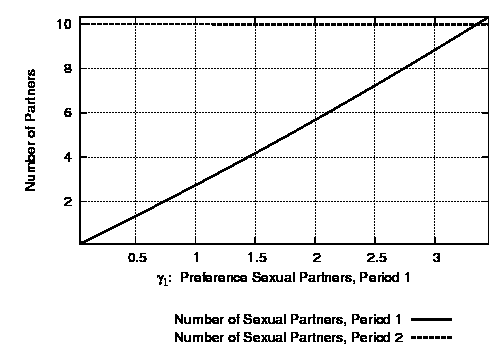
\includegraphics[scale=0.39]{images/mgamma1.png} & 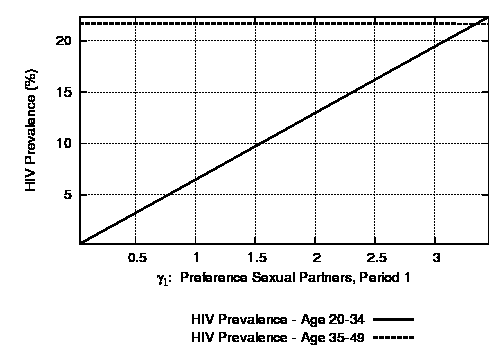
\includegraphics[scale=0.39]{images/hivgamma1.png} \\ \hline
\textbf{$\gamma_2$} & 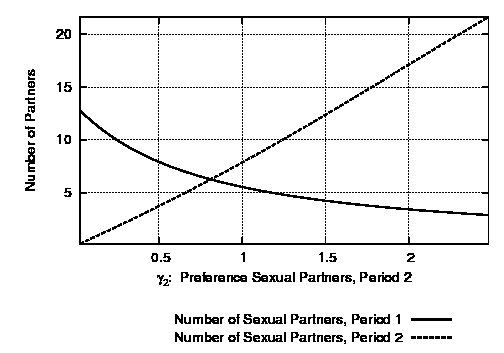
\includegraphics[scale=0.39]{images/mgamma2.png} & 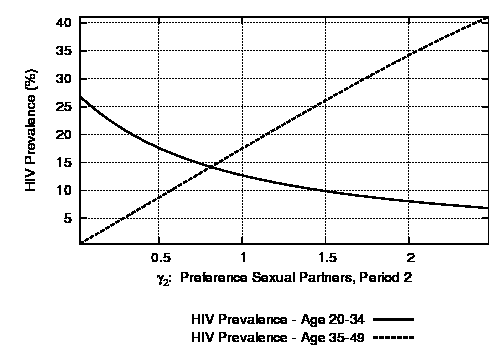
\includegraphics[scale=0.39]{images/hivgamma2.png} \\ \hline
\textbf{$\alpha$} & 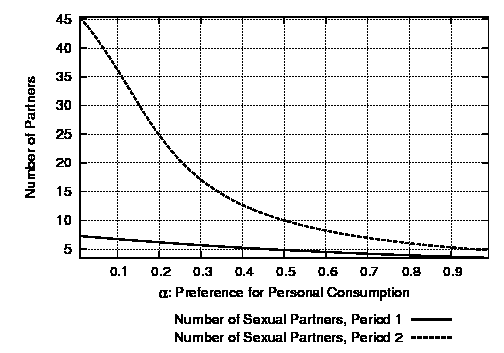
\includegraphics[scale=0.39]{images/malpha.png} & 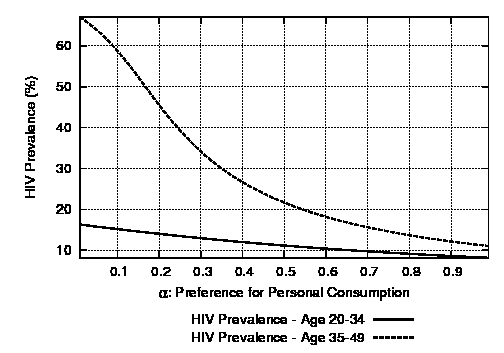
\includegraphics[scale=0.39]{images/hivalpha.png} \\ \hline
\textbf{$\nu$} & 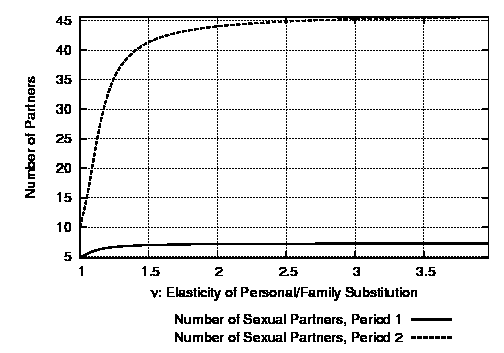
\includegraphics[scale=0.39]{images/msub.png} & 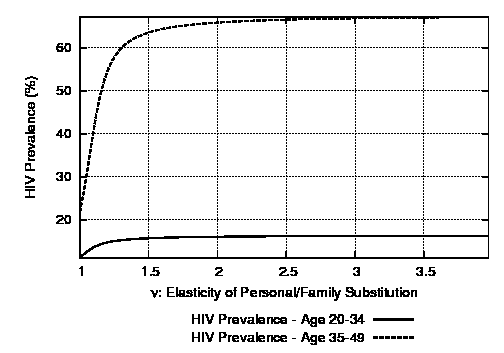
\includegraphics[scale=0.39]{images/hivsub.png} \\\hline
\multicolumn{3}{p{6.3in}}{
\footnotesize{
These plots illustrate the utility maximizing choice for the number of sexual partners, and the resulting HIV prevalence rates, for ranges of calibrations for the preference parameters.  For each plot, all other parameters are held constant at the values reported in Table \ref{tb:parms}. Parameters:
$\gamma_1$, Preference for Sexual Partners during ages 20-34;
$\gamma_2$, Preference for Sexual Partners during ages 35-49;
$\alpha$, Preference for Personal Consumption over Family Consumption;
$\nu$, Elasticity of Substitution Between Personal and Family Consumption.
}
}
\end{tabular}
\end{center}
\end{figure}


\begin{figure}
\begin{center}
\caption{Dynamics of Risky Behavior and HIV: Transmission Parameters}\label{fg:trans}
\vspace*{1pc}
\begin{tabular}{c|V|V@{}}
Parameter & Number of Sexual Partners & HIV Prevalence \\ \hline
\textbf{$h$} & 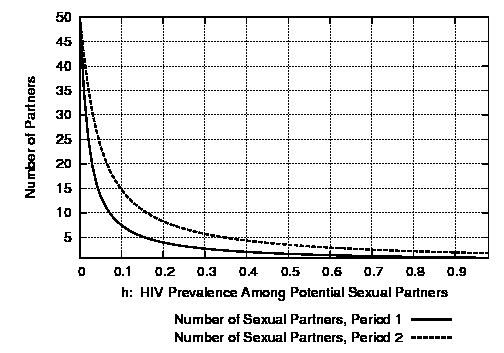
\includegraphics[scale=0.39]{images/mh.png} & 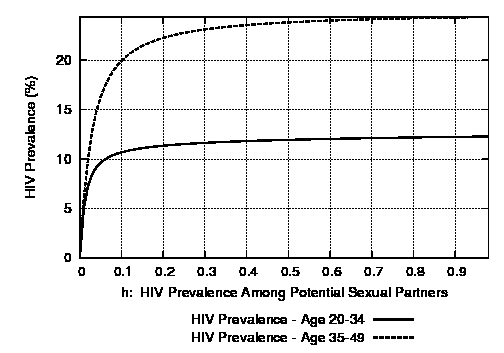
\includegraphics[scale=0.39]{images/hivh.png} \\ \hline
\textbf{$\tau$} & 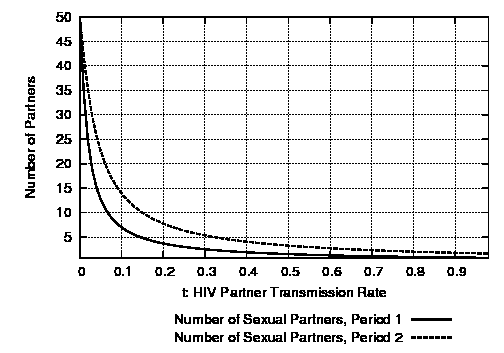
\includegraphics[scale=0.39]{images/mt.png} & 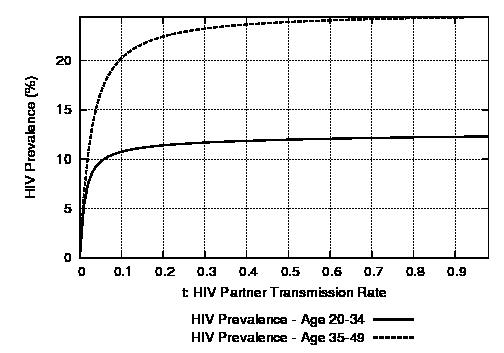
\includegraphics[scale=0.39]{images/hivt.png} \\ \hline
\multicolumn{3}{p{6.3in}}{
\footnotesize{
Note: These plots illustrate the utility maximizing choice for the number of sexual partners, and the resulting HIV prevalence rates, for ranges of calibrations for parameters $h$ and $\tau$, the HIV prevalence rate among potential sexual partners and the female-to-male HIV transmission rate, respectively.  For each plot, all other parameters are held constant at the values reported in Table \ref{tb:parms}.
}
}
\end{tabular}
\end{center}
\end{figure}


\begin{figure}
\begin{center}
\caption{Dynamics of Risky Behavior and HIV: Income, Life Expectancy, and Life Insurance}\label{fg:lifey}
\vspace*{1pc}
\begin{tabular}{c|V|@{}V@{}}
Parameter & Number of Sexual Partners & HIV Prevalence \\ \hline
Income & 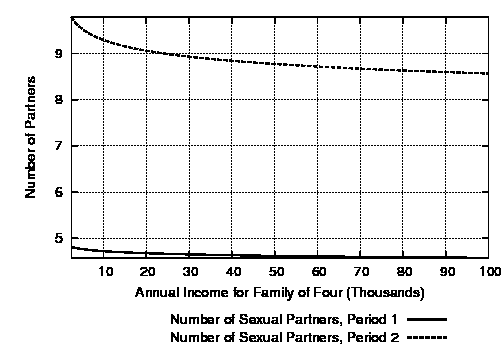
\includegraphics[scale=0.37]{images/mgdp.png} & 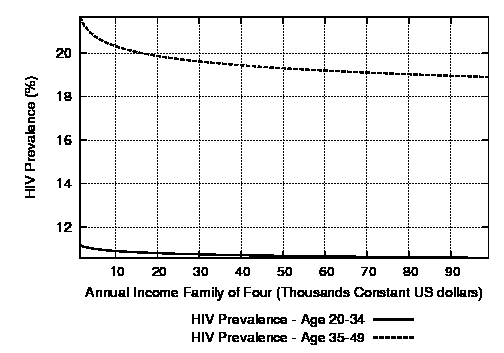
\includegraphics[scale=0.37]{images/hivgdp.png} \\ \hline
\begin{tabular}{p{0.8in}}Non-AIDS\newline Life\newline Expectancy\\\end{tabular} & 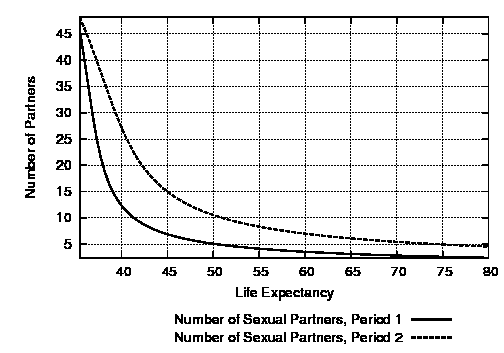
\includegraphics[scale=0.37]{images/mlife.png} & 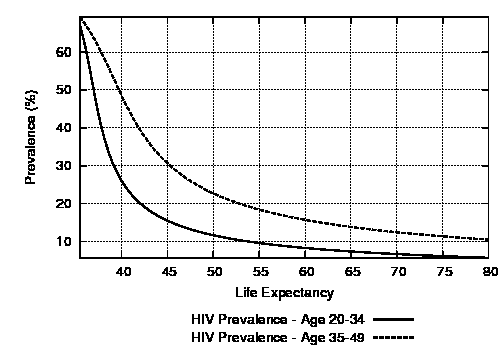
\includegraphics[scale=0.37]{images/hivlife.png} \\ \hline
\begin{tabular}{p{0.8in}}Life\newline Insurance\newline Payout\\\end{tabular} & 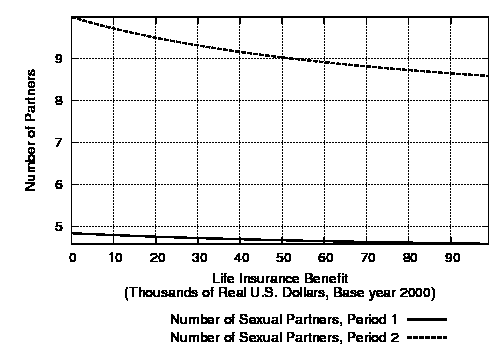
\includegraphics[scale=0.37]{images/mB.png} & 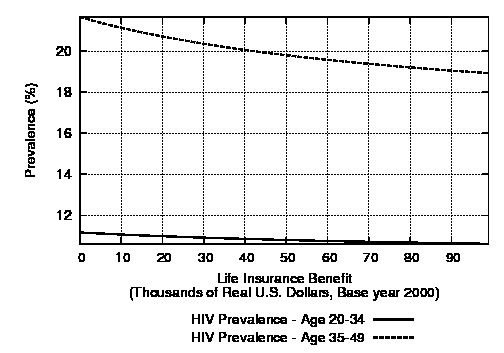
\includegraphics[scale=0.37]{images/hivB.png} \\ \hline
\multicolumn{3}{p{6.3in}}{
\footnotesize{
Note: The first two rows of plots demonstrate how income and life expectancy impact the utility maximizing choice for the number of sexual partners, and the resulting HIV prevalence rates.  For these plots, all other parameters are held constant at the values reported in the first column of Table \ref{tb:parms}.  The third row sets all parameters including life expectancy and income back to the baseline values, and illustrates how the utility maximizing number of sexual partners and HIV prevalence rates for various levels of life insurance paid out if death is not the result of AIDS.
}
}
\end{tabular}
\end{center}
\end{figure}


\begin{figure}
\begin{center}
\caption{Interaction of Income and Life Expectancy}\label{fg:incomelife}
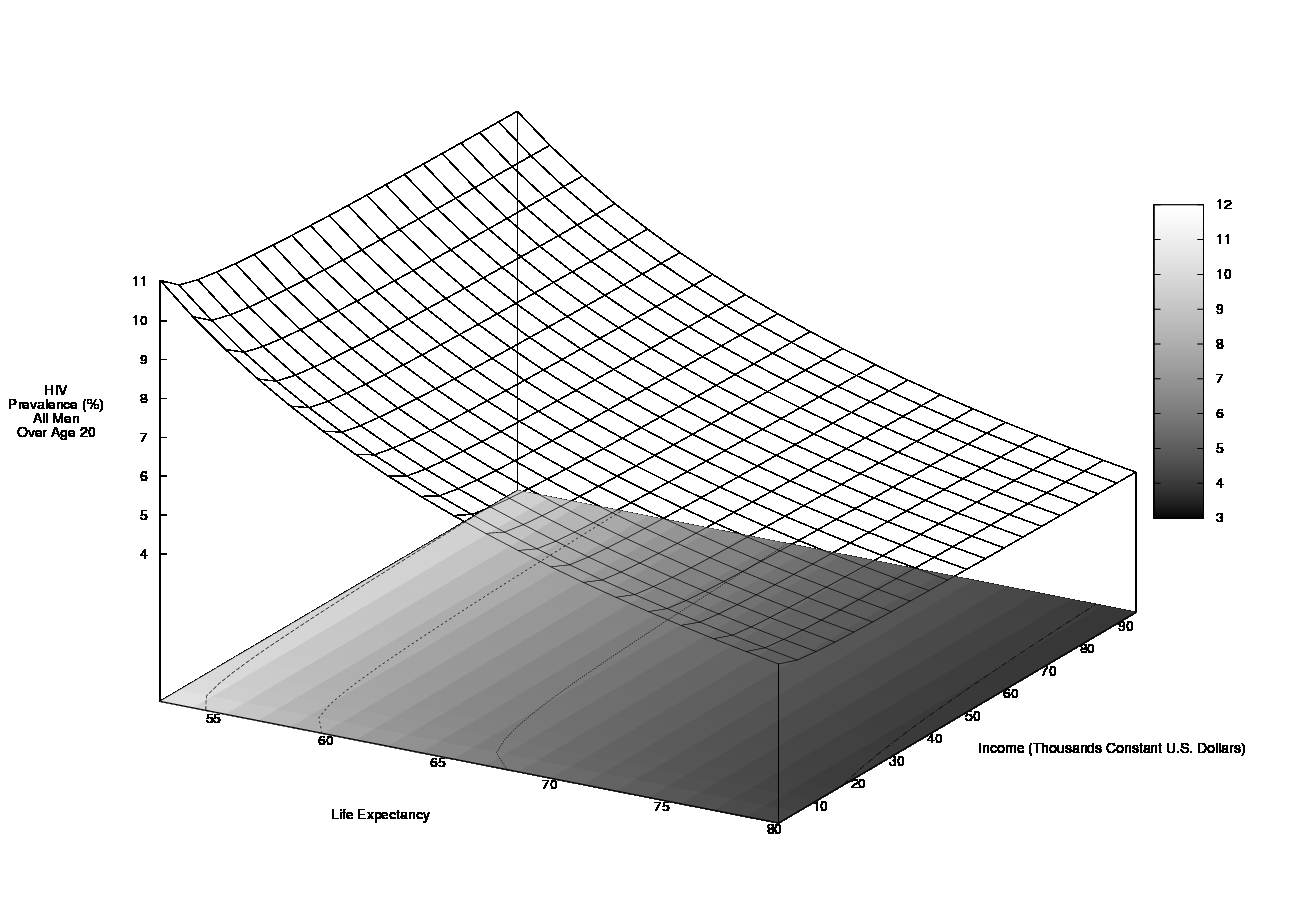
\includegraphics[scale=0.33]{images/hiv_gdplife.png}\\
\parbox{5.5in}{\footnotesize{Note: This figure illustrates the effect of the interaction of prolonged life expectancy and increased income on HIV prevalence among adult males.  The base of the three-dimensional graph contains contour lines and shading to help illustrate the height of the figure.  The lighter is the shading at a particular point, the taller is the figure at this point.  The greater descent from right to left than front to back indicates that increased life expectancy is a greater deterrent to risky behavior than increased income.  The lowest point on the graph (darkest shading) in the rear-left-hand corner indicates moving a country like Zambia into a situation with high life expectancy \textit{and} high income will result in a reduction of HIV prevalence among adult males from 11.9\% to almost 3\%.}}
\end{center}
\end{figure}

\begin{figure}
\begin{center}
\caption{Sensitivity of the Income Effect to the Elasticity of Substitution}\label{fg:incomenu}
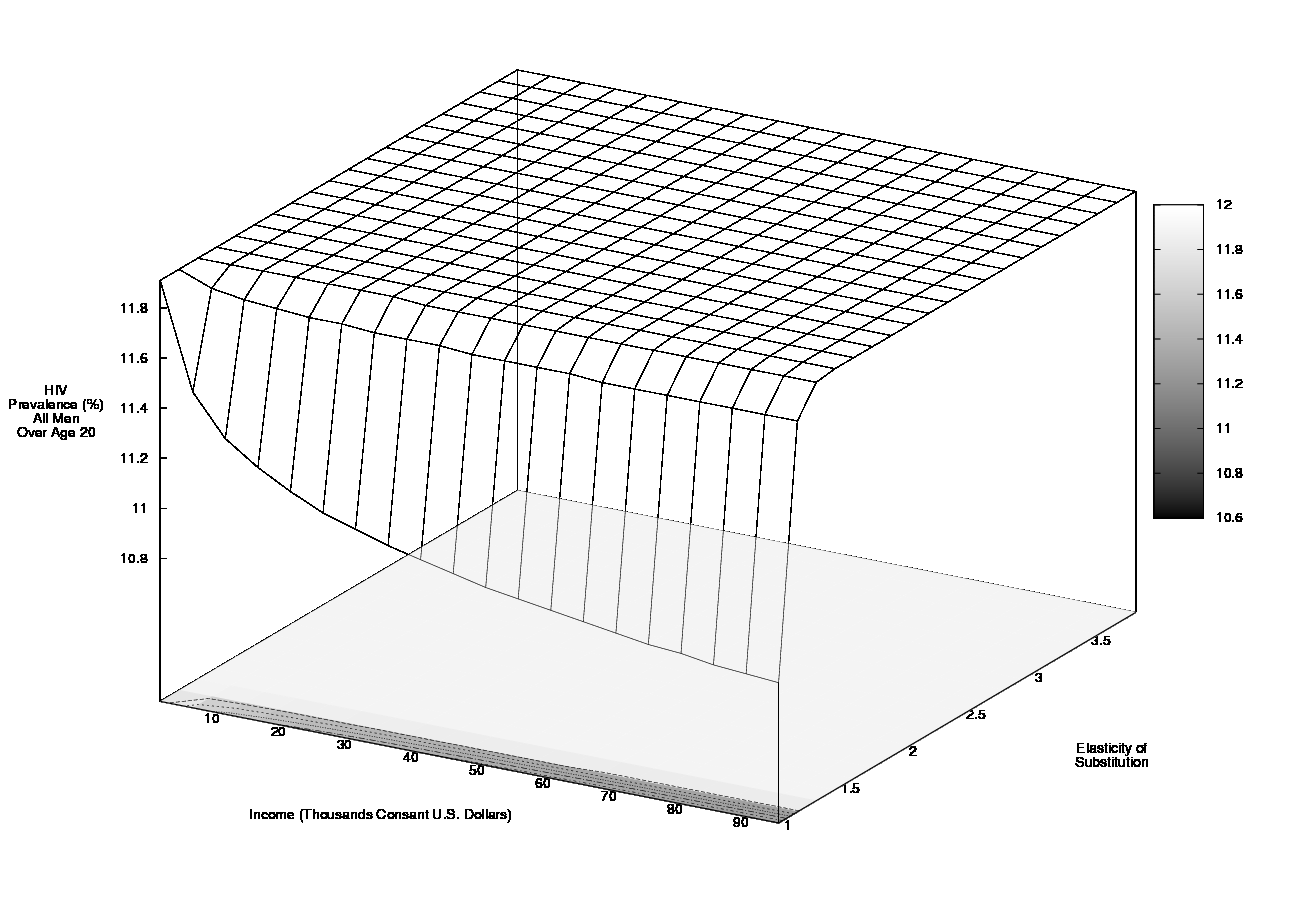
\includegraphics[scale=0.33]{images/hiv_gdpsub.png} \\
\parbox{5.5in}{\footnotesize{Note: This figure illustrates the deterrence effect of increasing income on HIV prevalence for various calibrations for $\nu$, the elasticity of substitution between personal and family consumption.  The base of the three-dimensional graph contains contour lines and shading to help illustrate the height of the figure.  The lighter is the shading at a particular point, the taller is the figure at this point.  For each value of $\nu$, a search is conducted for new calibrations of $\gamma_1$ and $\gamma_2$ so that at the baseline level of income, the resulting HIV prevalence rates among males 20-34 and 35-49 matches the data reported in Table \ref{tb:data}, which leads the model to predict the HIV prevalence rate among all adult males is 11.9\%.  The graph implies a very small response to risky behavior when $\nu=1$, and the deterrence effect of higher income completely disappears as personal and family consumption become substitutes ($\nu>1$).}}
\end{center}
\end{figure}

\begin{figure}
\begin{center}
\caption{Sensitivity of Life Expectancy Effect to the Elasticity of Substitution}\label{fg:lifenu}
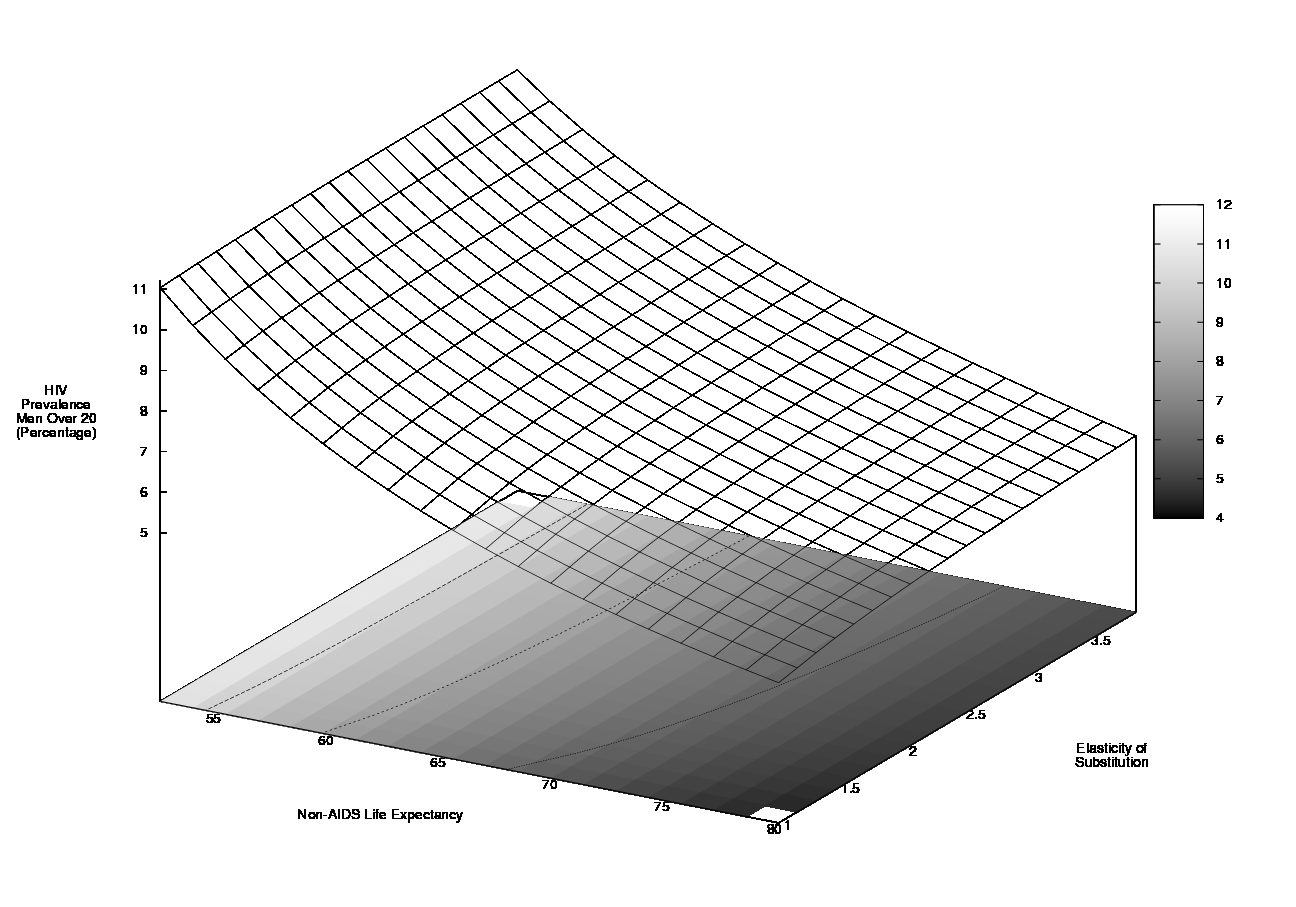
\includegraphics[scale=0.33]{images/hiv_lifesub.png} \\
\parbox{5.5in}{\footnotesize{Note: This figure illustrates the deterrence effect of increasing life expectancy on HIV prevalence for various calibrations for $\nu$, the elasticity of substitution between personal and family consumption.  The base of the three-dimensional graph contains contour lines and shading to help illustrate the height of the figure.  The lighter is the shading at a particular point, the taller is the figure at this point.  For each value of $\nu$, a search is conducted for new calibrations of $\gamma_1$ and $\gamma_2$ so that at the baseline level of life expectancy, the resulting HIV prevalence rates among males 20-34 and 35-49 matches the data reported in Table \ref{tb:data}, which leads the model to predict the HIV prevalence rate among all adult males is 11.9\%.  The graph shows there are quantitatively small differences in the deterrence effect over a large range for $\nu$.  The lowest point on the graph (and therefore the darkest shading on the base) occurs when $\nu$ is small, indicating that the deterrence effect is largest when personal and family consumption are not substitutes.}}
\end{center}
\end{figure}

\begin{figure}
\begin{center}
\caption{Sensitivity of Life Insurance Effect to the Elasticity of Substitution}\label{fg:insnu}
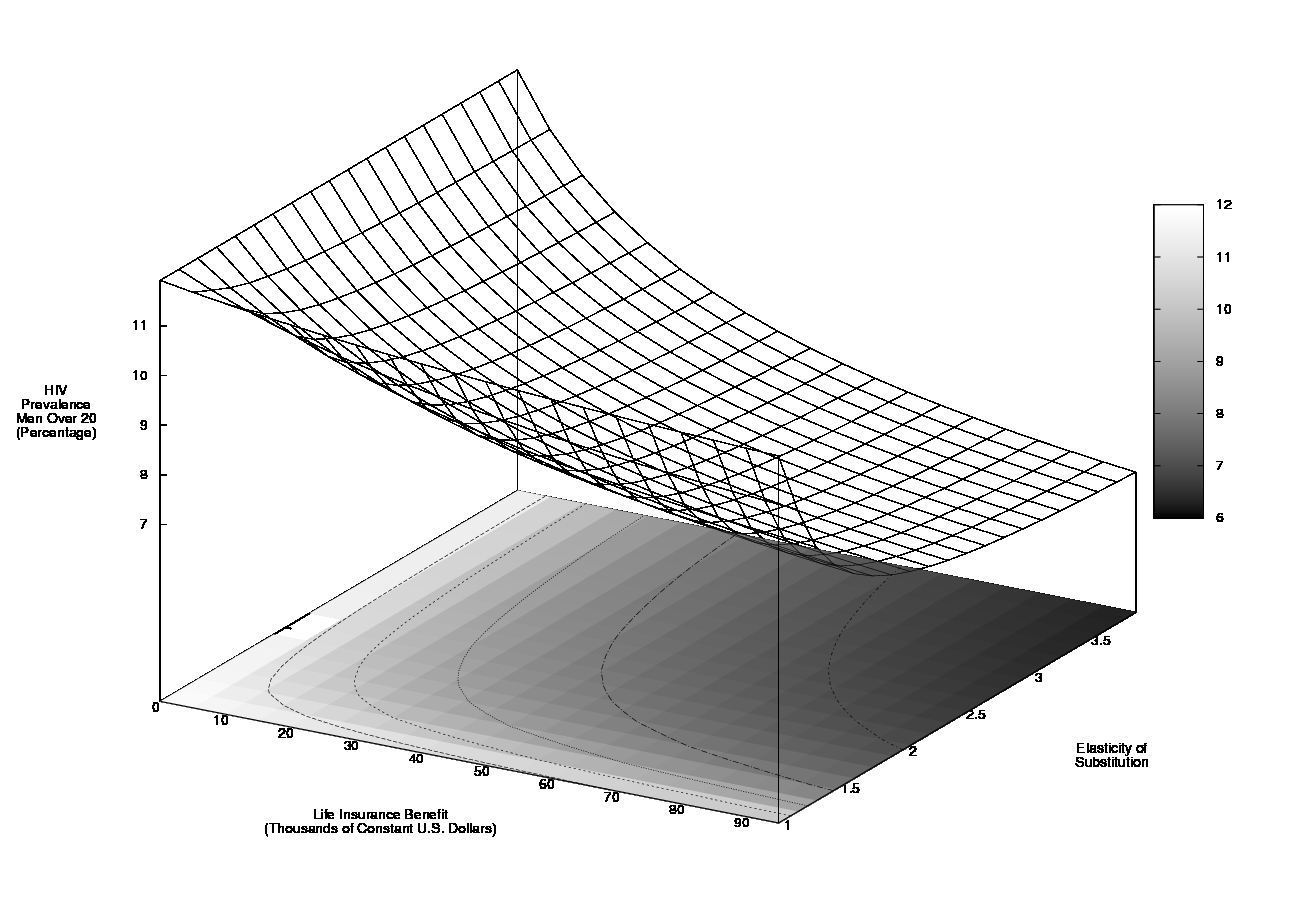
\includegraphics[scale=0.33]{images/hivBsub.png} \\
\parbox{5.5in}{\footnotesize{Note: This figure illustrates the deterrence effect of increasing life insurance benefits (paid out for any premature non-HIV related death) on HIV prevalence for various calibrations for $\nu$, the elasticity of substitution between personal and family consumption.  The base of the three-dimensional graph contains contour lines and shading to help illustrate the height of the figure.  The lighter is the shading at a particular point, the taller is the figure at this point.  For each value of $\nu$, a search is conducted for new calibrations of $\gamma_1$ and $\gamma_2$ so that at a baseline of zero life insurance benefits, the resulting HIV prevalence rates among males 20-34 and 35-49 matches the data reported in Table \ref{tb:data}, which leads the model to predict the HIV prevalence rate among all adult males is 11.9\%.  The graph shows a quick, steep decline in height moving front to back, indicating that as personal and family consumption becomes substitutable, life insurance benefits become a more effective deterrence.  For the highest levels for $\nu$, a life insurance benefit of \$100,000 can reduce HIV prevalence among all adult males to about 6\%. }}
\end{center}
\end{figure}

\begin{figure}
\begin{center}
\caption{Response to HIV Prevalence to Various Life Insurance Availabilities}\label{fg:available}
\begin{tabular}{cc}
\parbox{2.5in}{\begin{center}Payout Available if Death Follows Periods 1, 2, or 3\end{center}} & \parbox{2.5in}{\begin{center}Payout Available if Death Follows Periods 2 and 3\end{center}} \\
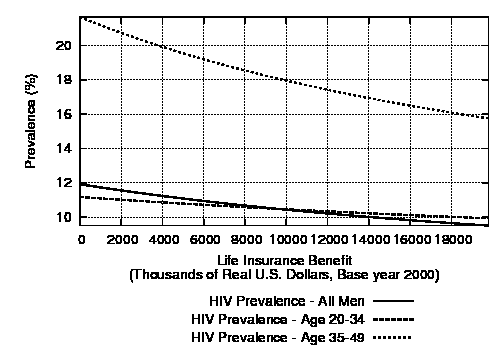
\includegraphics[scale=0.44]{images/hivB111.png} & 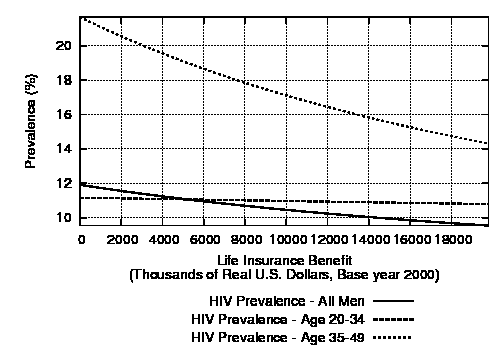
\includegraphics[scale=0.44]{images/hivB011.png} \\
\parbox{2.5in}{\begin{center}Payout Available if Death Follows Period 3\end{center}} & \parbox{2.5in}{\begin{center}Payout Available if Death Follows Period 2\end{center}} \\
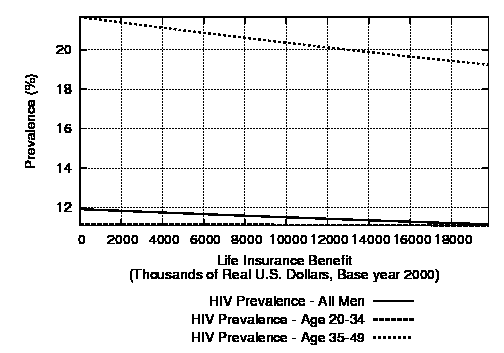
\includegraphics[scale=0.44]{images/hivB001.png} & 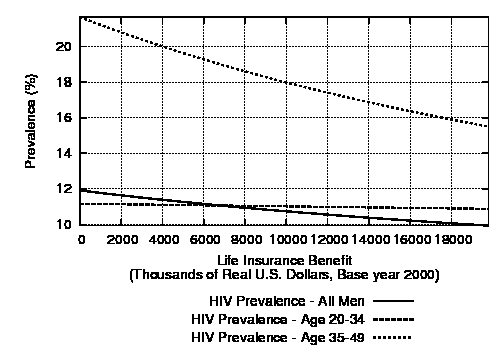
\includegraphics[scale=0.44]{images/hivB010.png} \\
\end{tabular}
\parbox{6.5in}{\footnotesize{Note: These figures illustrate the dynamics of the deterrence effect of a life insurance benefit up to \$20,000 when limiting the payouts only to deaths occurring at specific ages.}}
\end{center}
\end{figure}

\begin{figure}
\begin{center}
\caption{Deterrence Effect of Life Insurance by Country}\label{fg:bycountry}
\vspace*{1pc}
\begin{tabular}{cc}
Zambia  & Kenya \\
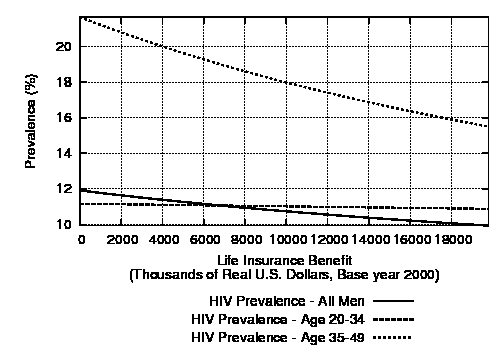
\includegraphics[scale=0.44]{images/hivB010_Zambia.png} & 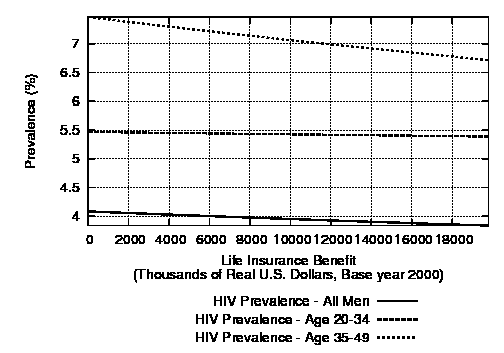
\includegraphics[scale=0.44]{images/hivB010_Kenya.png} \\
Tanzania & Ethiopia \\
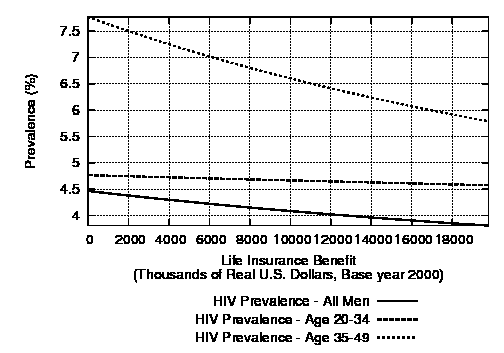
\includegraphics[scale=0.44]{images/hivB010_Tanzania.png} & 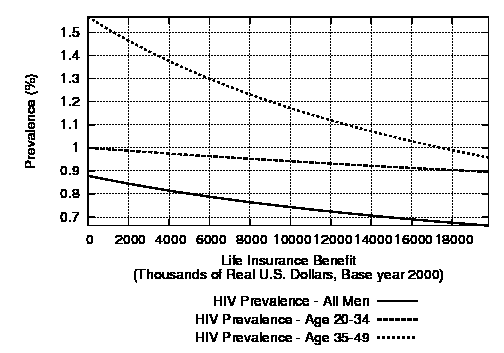
\includegraphics[scale=0.44]{images/hivB010_Ethiopia.png} \\
\multicolumn{2}{c}{Rwanda} \\
\multicolumn{2}{c}{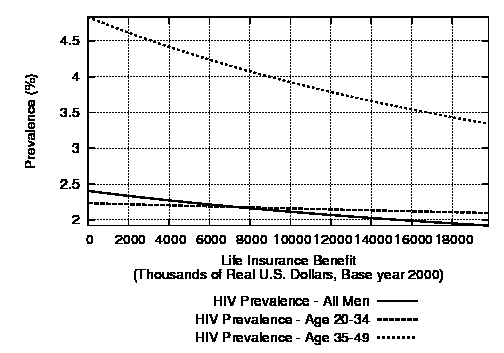
\includegraphics[scale=0.44]{images/hivB010_Rwanda.png}} \\\\
\end{tabular}
\parbox{6.5in}{\footnotesize{Note: These figures illustrate the dynamics of the deterrence effect of a life insurance benefit up to \$20,000 when life insurance benefit is only available if a non-HIV related death occurs immediately following period 2 (age 50).}}
\end{center}
\end{figure}

\end{document}






% LocalWords:  de Araujo Poudre Crosse capita JEL additivity substitutability
% LocalWords:  Inada CES kremer eo
